% main_co2_nature_20260926.tex  (2026-09-26: Junya Estimation comments applied; airport regressions removed per
%   Junya's Overleaf comment; validation table and SCC table moved to Extended Data; Longfei figures (Figure1,
%   Figure2 panels a,b, ED_Fig1-4) with Ray's SAF figure as Fig. 3; abstract <= 200 words; Methods <= 3,000 words with
%   inventory and GACI details in Supplementary Notes 2-3; Extended Data ordered by first citation)
% Main displays: Tables 1-3 (main, decomposition, spatial) and Figs 1-3 (decomposition/heterogeneity, attribution, SAF).
% --- history ---
% main_co2_nature_20260908.tex  (candidate, 2026-09-08)
% Built by 36_apply_comments_20260908.py from Downloads/main_co2_nature_20260906 (1).tex
% (user copy with the new Chunan/Fangyu Methods: flight-level emissions, allocation,
% validation incl. BTS 3.84%/+0.76%, GACI) with the 09-08 changes:
%   - Main section replaced by Yifu's rewrite (Main_YO_Sep7.docx); natbib author-year,
%     refs_co2.bib (14 entries); old Main kept in FINAL_20260908/_old_main_section_20260906.tex
%   - Table 1: intensity column removed (reported in Table 2); prose reference updated
%   - Extended Data Table 1: Panels D-E (unrestricted split) removed; note rewritten
% Inference: standard errors clustered by country throughout (09-03 decision).
%   - 09-09 (user markers): bunker attribution-mismatch passage removed and the
%     airport passage cut to one regression result and one emissions result;
%     ED Figs 'levels', 'mismatch', 'effcurve' and 'rfquintile' deleted. The
%     airport regressions (ED Table 'airport_het', Supplementary Table
%     'airport_iv', Methods airport subsection) and the concentration result
%     (ED Fig 'airportconc', ED Table 'airport_conc') are retained.
% Main displays: Tables 1-4 (main, decomposition, spatial, SCC) and Figs 1-3
% (heterogeneity, attributed map, SAF). Extended Data: tables 1-13, figures 1-8;
% Supplementary Note 1 and Supplementary tables 1-3. [TODO cite] markers remain outside Main; compile on Overleaf.
\documentclass[12pt]{extarticle}
\usepackage[margin=2.2cm]{geometry}
\usepackage{setspace}
\usepackage{etoolbox}
\doublespacing
% tables, notes and captions stay single spaced for readability
\AtBeginEnvironment{table}{\singlespacing}
\AtBeginEnvironment{figure}{\singlespacing}
\usepackage{amsmath,graphicx,booktabs,threeparttable,float}
\usepackage{adjustbox}
\usepackage[authoryear,round]{natbib}
\title{How Much Does Air Connectivity Increase Aviation CO$_2$?}
\author{[Author list and order to be confirmed]}
% Contributors (alphabetical, order not decided): Fangyu Cao, Lisa Hsieh, Jinwoo Lee, Junya Kumagai, Longfei Zheng, Ray (NTU), Sunbin Yoo, Chunan Wang, Yifu Ou.
\date{Nature-format draft, 26 September 2026}
\begin{document}
\maketitle

\begin{abstract}
\noindent Air connectivity is an explicit object of national policy, yet its
carbon consequences have not been estimated causally at the global level.
Here we construct flight-stage-resolved CO$_2$ for more than 6{,}000
airports over 1996--2023 from schedule data, match it to a global panel of
airport connectivity, and identify the effect of connectivity on emissions
with an instrument based on each country's air-market-access exposure to
global aviation growth. A one percent increase in
connectivity raises national aviation CO$_2$ by 5.3\%, an elasticity that does
not depend on how emissions are allocated across countries. The response comes from flight frequency: flights rise by
6.8\%, aircraft size and stage length do not rise, and the 0.3\% decline in
emissions per seat-kilometre offsets little of it. The elasticity is concentrated in low-income, newly connecting
countries and describes the take-off stage of network development.
Emissions also respond to contiguous neighbours' connectivity, with a
neighbour elasticity of 1.1 to 2.1 and a network-wide effect of 5.6.
Connectivity growth since 1996 accounts for 41\% (349 Mt) of 2023 aviation
CO$_2$, an annual external cost of \$18 billion to \$66 billion, and only
sustained fuel switching, not the efficiency gains of network development,
reverses this growth.
\end{abstract}

%=======================================================================
\section*{Main}
%=======================================================================
Air connectivity has become an important part of economic and transport
policy. Governments expand airport capacity, support new routes and
negotiate air-service agreements to improve access to the global air
network \citep{fageda2018,piermartini2013}. A large body of literature
links better connectivity to trade, tourism, investment, and regional
development \citep{lenaerts2021,zhang2020,amico2026}, making network expansion
particularly important for countries with limited global access. However,
the climate implications of air connectivity development are less clear.
Aviation remains difficult to decarbonize because large-scale
electrification is not expected in the near term, while continued growth
in air travel can offset gains from more efficient aircraft and
lower-carbon fuels \citep{bergero2023,sacchi2023}. As countries continue
to expand their air networks, a basic question emerges: what happens to
carbon emissions when air connectivity improves?

The answer depends on how connectivity changes aviation activity. On the
one hand, better connections can open new destinations and induce trips
that would otherwise not occur \citep{koo2017,piermartini2013}. On the
other hand, they can also change how those trips are served. Changes in
network structure can alter flight frequency, aircraft size, and routing,
with potentially offsetting effects on operating and environmental
efficiency \citep{brueckner2004,pels2021}. These changes can work in
opposite directions. More aviation activity raises total emissions, while
greater efficiency lowers the emissions associated with each unit of
travel. Evidence from other transport settings shows that induced demand
can offset some of the environmental gains from improved efficiency
\citep{hymel2010,ou2024}. The net carbon effect of connectivity is
therefore an empirical question. So is the source of that effect: whether
emissions change because airlines operate more flights, use different
aircraft, fly different distances, or provide transport more efficiently.

Existing research has not resolved this question. Studies of air
connectivity have focused mainly on its economic benefits, linking better
access to trade, tourism, productivity and regional development
\citep{lenaerts2021,zhang2020}, while research on aviation
decarbonization has focused on travel demand, aircraft and operational
efficiency, and lower-carbon fuels \citep{bergero2023,dray2022}. Much
less is known about how the development of the air network itself shapes
aviation activity and emissions. Estimating this effect is difficult
because causality can run in both directions. For example, while airlines
add routes and flights in response to growing demand, better connections
can also generate additional travel \citep{koo2017,pitfield2010}. Income,
trade, and tourism can further affect both network expansion and aviation
activity \citep{vandevijver2014,lenzen2018}. These sources of endogeneity can bias
estimates based on observed changes in connectivity. Therefore,
identifying the average causal effect of connectivity requires variation
that is not driven by local travel demand. This gap in causal evidence on
the carbon effects of air connectivity motivates our study.

However, the average effect alone provides an incomplete picture of the
carbon consequences of air connectivity. First, the carbon effect may
change as air networks develop. New connections can generate substantial
new activity in countries with sparse networks, while the same increase in
connectivity may have a smaller effect once networks are well developed.
Therefore, the carbon effect of connectivity may depend on the stage of
network development. Second, the effects may extend beyond the country
where connectivity expands. Air transport operates as an international
network, so greater connectivity in one country can change aviation
activity in neighbouring countries. Emissions associated with network
growth may also be concentrated in particular airports rather than spread
evenly across the network. These differences matter for understanding
when and where the carbon consequences of network expansion are greatest.

In this study, we address three questions. First, how does air
connectivity affect aviation CO$_2$, and through which changes in
aviation activity and efficiency? Second, how does the effect change as
air networks develop? Third, how are the carbon effects of connectivity
distributed across the air network, and do they extend across national
borders? We answer these questions using a global panel of air
connectivity and flight-stage-resolved CO$_2$ emissions from more than
6{,}000 airports between 1996 and 2023. To address endogeneity, we use a
shift-share instrumental-variable design based on countries'
predetermined exposure to global aviation expansion.

Our results reveal a large positive effect of air connectivity on
aviation CO$_2$, particularly during the ``take-off'' stages of network
development. Our main estimate indicates that a 1\% increase in
connectivity increases aviation CO$_2$ by about 5.3\%, driven primarily
by a roughly 7\% increase in flight frequency. Aircraft size, flight
distance, and carbon intensity decline slightly, but these changes are
not statistically significant. The effect on emissions is largest in
countries with lower initial income and connectivity and declines as
networks mature. The effects also extend across national borders, while
emissions associated with network growth are concentrated in a small
share of airports. These findings show that network expansion increases
aviation emissions mainly by generating additional flying, while
accompanying efficiency gains are too small to offset this growth.
Therefore, accounting for network-driven growth in aviation activity is
important for assessing pathways to aviation decarbonization.

%=======================================================================
\section*{Results}
%=======================================================================
\subsection*{The emissions elasticity of connectivity is positive}
We begin with the estimated elasticity of national aviation CO$_2$ with respect to connectivity and
its stability across measurement choices, controls and periods
(Table~\ref{tab:main}). A one percent increase in air connectivity raises national aviation CO$_2$
by 5.35\% (Table~\ref{tab:main}). The estimate is
robust in three respects. It remains positive under every way of
aggregating airport connectivity to the country level and stays between
5.3 and 5.7 across the rules for allocating emissions to countries
(Table~\ref{tab:main}; Extended Data Table~\ref{tab:alloc}). It stays
between 4.4 and 4.7 when income, trade, urbanization, investment and
tourism are controlled for, so it is not a development effect in disguise
(Extended Data Table~\ref{tab:exclusion}). It is positive in both halves
of the sample, at 5.6 in the network-expansion era before 2008 and 2.9 in
the mature-network era after 2010, so it halves as networks mature but
does not vanish (Extended Data Table~\ref{tab:temporal} and Extended Data
Fig.~\ref{fig:ed_temporal_airport}a).

\begin{table}[H]
\centering
\caption{Air connectivity and aviation CO$_2$: main results}
\label{tab:main}
\adjustbox{max width=\textwidth, max totalheight=0.9\textheight}{%
\begin{threeparttable}\footnotesize
\begin{tabular}{lccc}
\toprule
 & \multicolumn{1}{c}{Bunker CO$_2$} & \multicolumn{1}{c}{Intl.\ CO$_2$} & \multicolumn{1}{c}{Seat-km} \\
 & (1) & (2) & (3) \\
\midrule
\multicolumn{4}{l}{\textit{Panel A. OLS}} \\
ln GACI (cwm) & 3.388$^{***}$ & 3.526$^{***}$ & 3.684$^{***}$ \\
 & (0.364) & (0.358) & (0.398) \\
$N$ & 4,634 & 4,634 & 4,634 \\
\midrule
\multicolumn{4}{l}{\textit{Panel B. 2SLS, Feyrer instrument, capacity-weighted mean}} \\
ln GACI (cwm) & 5.347$^{***}$ & 5.192$^{***}$ & 5.641$^{***}$ \\
 & (1.076) & (1.043) & (1.194) \\
KP $F$ & 18.4 & 18.4 & 18.4 \\
$N$ & 4,634 & 4,634 & 4,634 \\
\midrule
\multicolumn{4}{l}{\textit{Panel C. 2SLS, GACI sum}} \\
ln GACI (sum) & 2.153$^{***}$ & 2.091$^{***}$ & 2.272$^{***}$ \\
 & (0.524) & (0.542) & (0.592) \\
KP $F$ & 14.0 & 14.0 & 14.0 \\
$N$ & 4,634 & 4,634 & 4,634 \\
\midrule
\multicolumn{4}{l}{\textit{Panel D. 2SLS, GACI max}} \\
ln GACI (max) & 4.548$^{***}$ & 4.416$^{***}$ & 4.798$^{***}$ \\
 & (0.841) & (0.845) & (0.955) \\
KP $F$ & 21.0 & 21.0 & 21.0 \\
$N$ & 4,634 & 4,634 & 4,634 \\
\midrule
\multicolumn{4}{l}{\textit{Panel E. 2SLS, GACI mean}} \\
ln GACI (mean) & 5.562$^{***}$ & 5.401$^{***}$ & 5.868$^{***}$ \\
 & (1.389) & (1.334) & (1.491) \\
KP $F$ & 29.3 & 29.3 & 29.3 \\
$N$ & 4,634 & 4,634 & 4,634 \\
\bottomrule
\end{tabular}
\begin{tablenotes}[flushleft]
\footnotesize
\item Notes: Country-year panel, 1996--2023. All specifications include country and year fixed effects, log population and log sea market access. Outcomes are in logs: total aviation CO$_2$ under the bunker convention (all cruise plus departure-side LTO assigned to the departure country), bunker CO$_2$ from international flights, and scheduled departing seat-kilometres; CO$_2$ per seat-km is in Table~\ref{tab:decomp}. Panels B--E instrument log GACI with the Feyrer interaction of the world aviation index and log 1996 air market access, with log sea market access as a control (Methods, equation~\ref{eq:feyrer}). Standard errors clustered by country in parentheses; the Kleibergen--Paap $F$ is cluster-robust. $^{***}$, $^{**}$, $^{*}$: significance at 1, 5, and 10\%.
\end{tablenotes}
\end{threeparttable}}
\end{table}

\subsection*{Where the elasticity comes from: frequency, not aircraft size
or efficiency}
We next ask where the elasticity comes from, by decomposing the
response into flights, aircraft size, stage length and carbon intensity
(Table~\ref{tab:decomp}). The variation that raises emissions by 5.35\% raises seat-kilometres by 5.64\%, so emissions per seat-kilometre fall by
0.29\%, an efficiency term not distinguishable from zero
(Table~\ref{tab:decomp}). Emissions therefore grow with the network
almost exactly as traffic does. Because national CO$_2$ is the product of
flights, seats per flight, kilometres per flight and CO$_2$ per
seat-kilometre, the four component elasticities sum to the total
(Methods, equations~\ref{eq:identity} and \ref{eq:decomp}). The response is a frequency response: flights rise by 6.8\% for a one percent gain in connectivity, whereas aircraft size,
stage length and carbon intensity each move by less than one percent and
not significantly (Fig.~\ref{fig:decomp_het}a). Traffic
expansion accounts for the whole of the emissions response and the
efficiency term offsets 6\% of it. The share of
landing-and-take-off emissions and the international share of traffic do
not move, and mediation analysis attributes 84 to 85\% of the effect
to flight frequency and traffic volume (Extended Data
Table~\ref{tab:mediation}).

\begin{table}[H]
\centering
\adjustbox{max width=\textwidth, max totalheight=0.9\textheight}{%
\begin{threeparttable}
\caption{Decomposition of the CO$_2$ elasticity on the accounting identity}
\label{tab:decomp}
\footnotesize
\begin{tabular}{lccc}
\toprule
 & Elasticity to GACI & s.e. & Share of total (\%) \\
\midrule
\multicolumn{4}{l}{\textit{Scale components}} \\
  Flights (frequency) & +6.760$^{***}$ & (1.367) & +126 \\
  Seats per flight (aircraft gauge) & -0.336 & (0.432) & -6 \\
  Km per flight (average stage length) & -0.782 & (0.569) & -15 \\
  \textbf{Subtotal: scale (seat-km)} & +5.641$^{***}$ & (1.194) & +106 \\
\multicolumn{4}{l}{\textit{Efficiency component}} \\
  CO$_2$ per seat-km (carbon intensity) & -0.294 & (0.286) & -6 \\
\midrule
  \textbf{Total CO$_2$ (equals Table~\ref{tab:main}, column 1)} & +5.347$^{***}$ & (1.076) & +100 \\
\midrule
\multicolumn{4}{l}{\textit{Composition margins (memo)}} \\
  LTO share of CO$_2$ & +0.037 & (0.069) & -- \\
  International share of seat-km & +0.019 & (0.115) & -- \\
\bottomrule
\end{tabular}
\begin{tablenotes}\footnotesize
\item Each row is a separate 2SLS regression of the log component on log GACI (capacity-weighted mean), instrumented by the Feyrer interaction, with log population and log sea market access, country and year fixed effects, and standard errors clustered by country; identical sample of 4,634 country-years, first-stage Kleibergen--Paap $F$ = 18.4. Because CO$_2$ = flights $\times$ seats per flight $\times$ km per flight $\times$ CO$_2$ per seat-km, the log elasticities add exactly to the total. Load factor is constant by construction (scheduled capacity) and cancels. Shares are component elasticity divided by the total. $^{***}$ $p<0.01$, $^{**}$ $p<0.05$, $^{*}$ $p<0.1$.
\end{tablenotes}
\end{threeparttable}}
\end{table}

\begin{figure}[H]
\centering
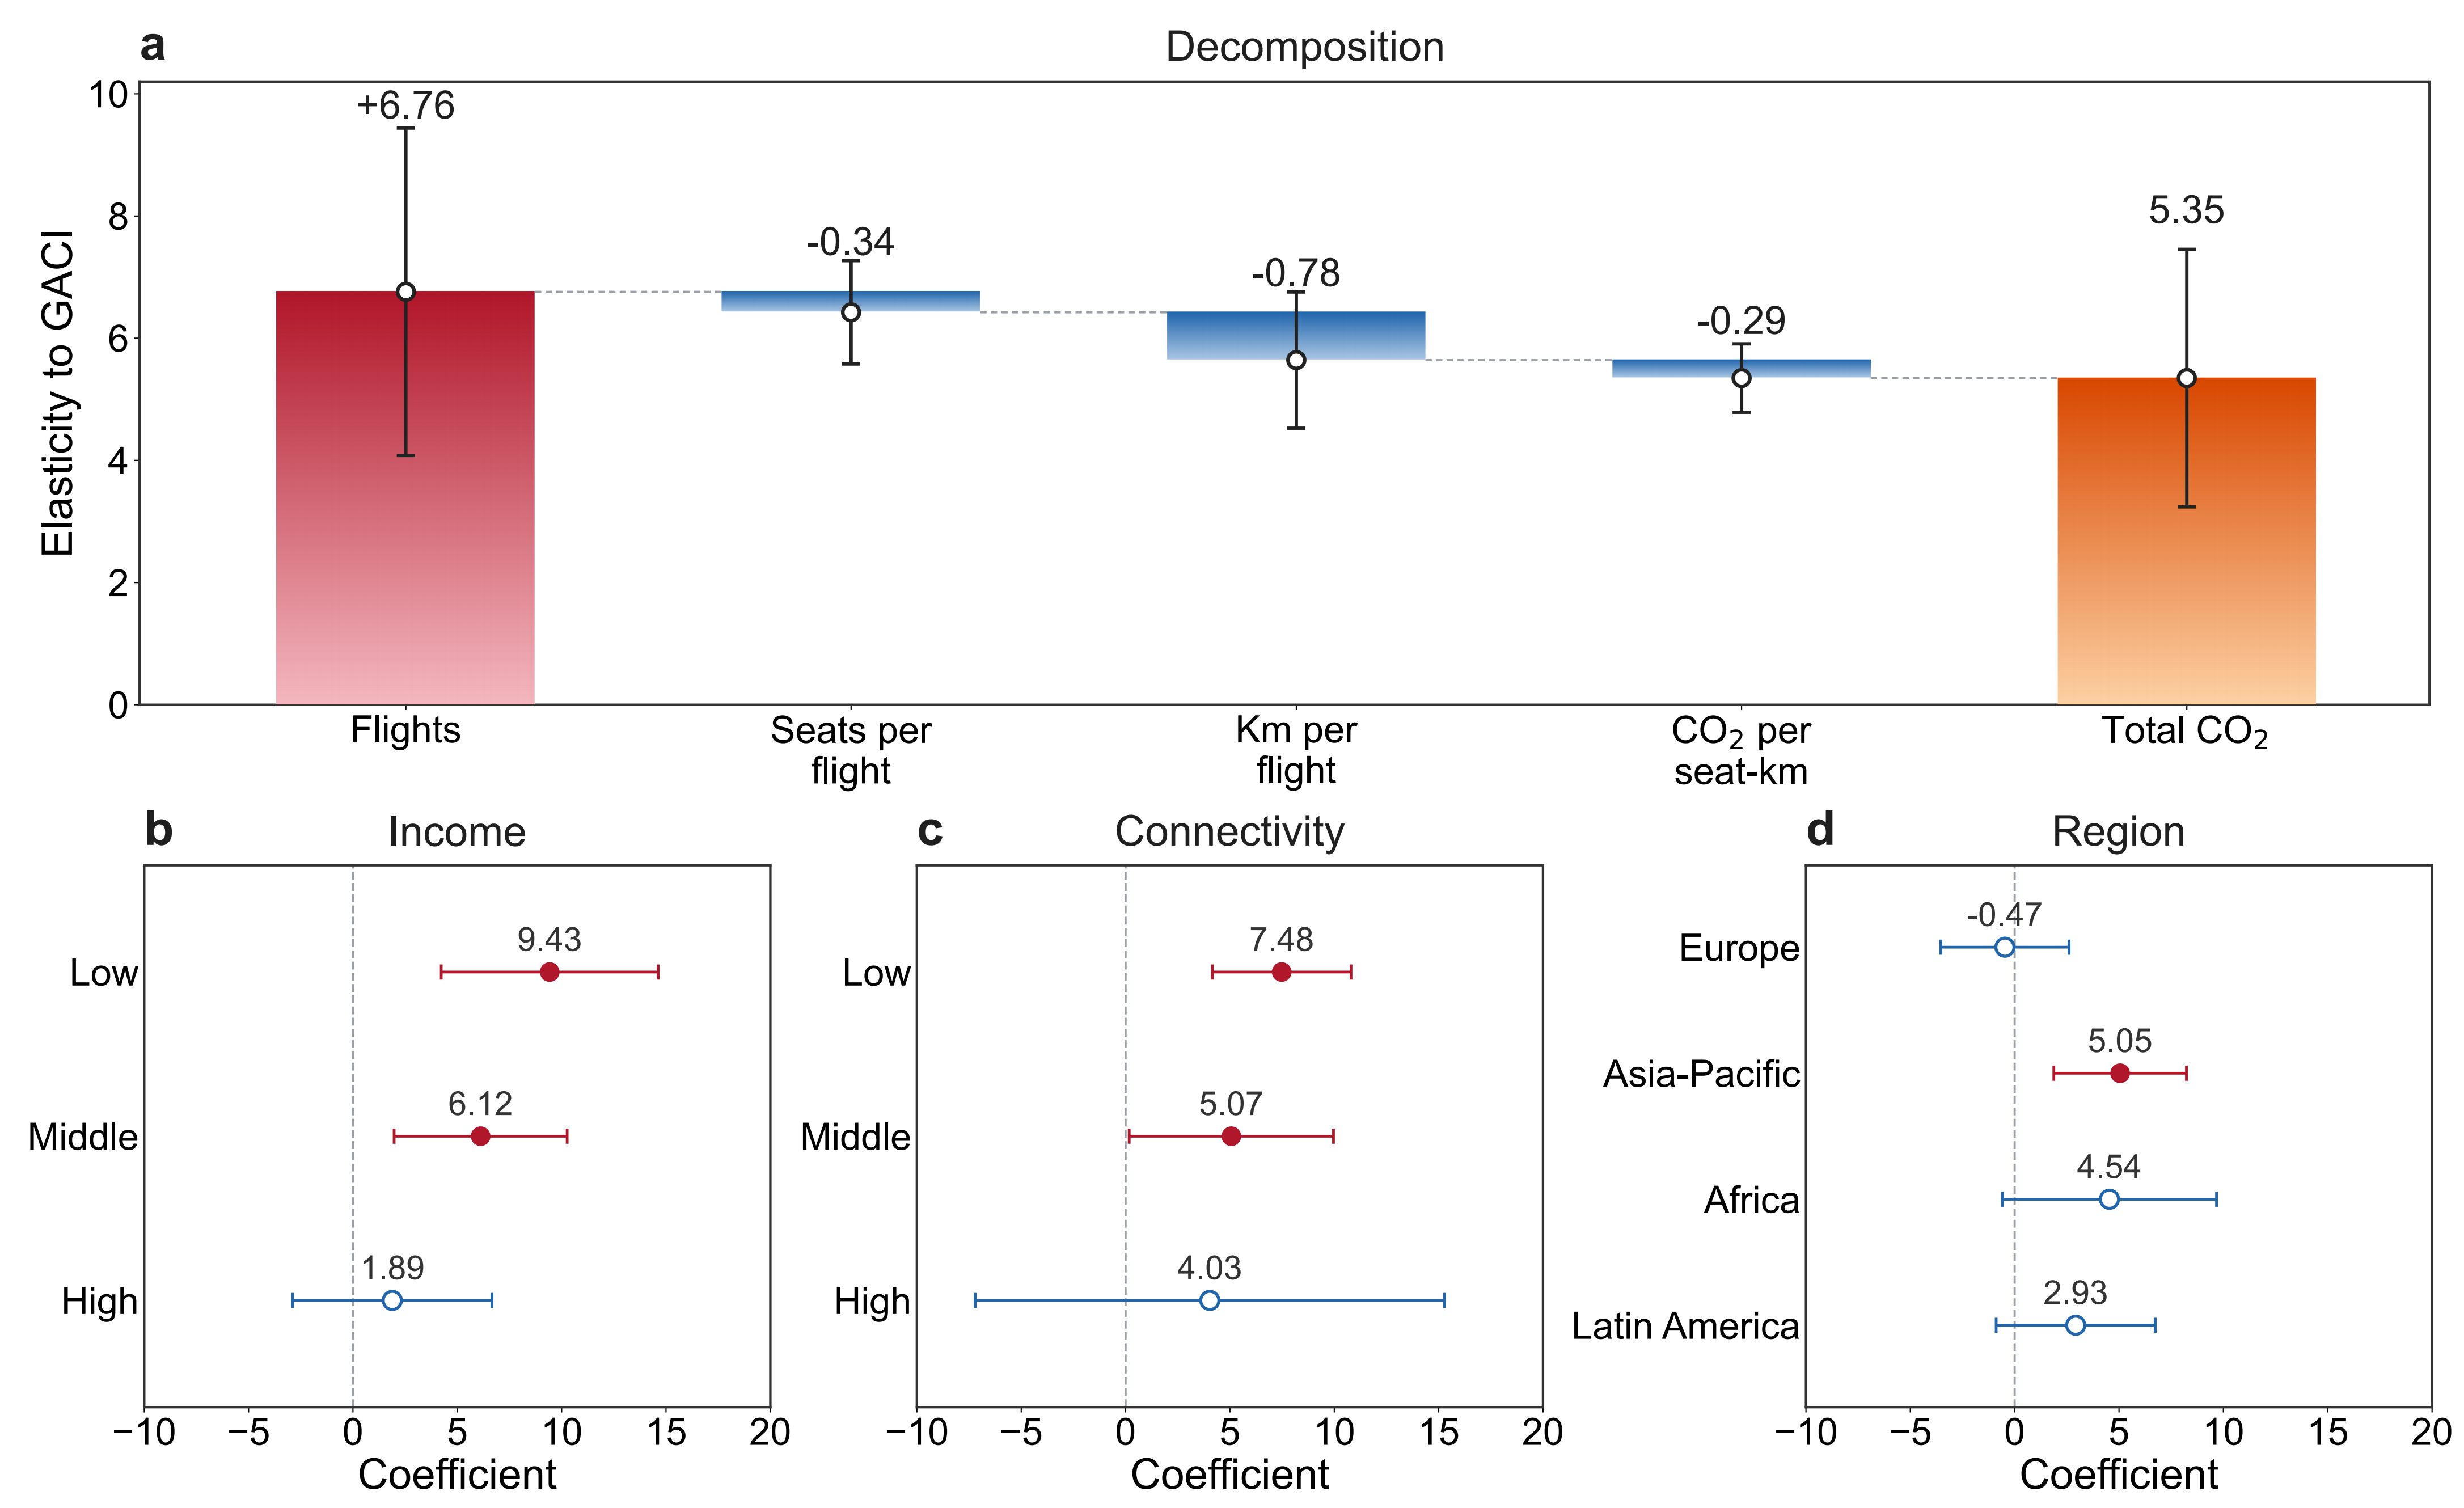
\includegraphics[width=0.98\textwidth]{Figure1.png}
\caption{\textbf{Decomposition and heterogeneity of the connectivity elasticity.} \textbf{a}, Decomposition of the elasticity of national aviation CO$_2$ on the accounting identity. Each bar is the 2SLS elasticity of one component with respect to connectivity (Feyrer instrument), and the four components add exactly to the total; the scale margin (the sum of the first three bars, seat-km) is 5.64 and the efficiency margin (CO$_2$ per seat-km) is $-$0.29. \textbf{b}--\textbf{d}, Split-sample 2SLS elasticities of total bunker CO$_2$ by 1996 income tercile (\textbf{b}), 1996 connectivity tercile (\textbf{c}) and region (\textbf{d}). Filled red markers denote $p<0.05$ and open blue markers $p\geq0.05$. The Middle East and North America are omitted as unidentified, and the high-connectivity tercile has a weak first stage (KP $F$ = 0.2). Bars are 95\% confidence intervals with standard errors clustered by country.}
\label{fig:decomp_het}
\end{figure}

The same pattern holds within income groups and across international and
domestic flying (Extended Data Table~\ref{tab:decomp_hetero}). In low-
and middle-income countries flights rise by about 8.5\% for a one
percent gain in connectivity, for total elasticities of 9.4 and 6.1; in
high-income countries the total is 1.9 and no component responds
significantly, additional frequency being offset by smaller aircraft and
shorter stages. International emissions respond with an elasticity of
5.2, carried by frequency, whereas domestic emissions do not respond.
Additional flights, not larger aircraft or longer routes, therefore carry
the response.

\subsection*{The elasticity is concentrated in newly connecting countries}
We then ask for whom the elasticity holds. This section splits the sample
by 1996 income, baseline connectivity and region (Fig.~\ref{fig:decomp_het}b--d)
and checks that the gradient survives in levels and in finer splits of the
baseline distribution (Extended Data).

The elasticity falls steeply with 1996 income and connectivity
(Fig.~\ref{fig:decomp_het}b,c and Extended Data Table~\ref{tab:hetero}). By
income it falls from 9.4 in the bottom tercile to 6.1 in the middle and
1.9 at the top; by baseline connectivity from 7.5 in the bottom tercile
to 5.1 in the middle, while the top tercile is unidentified (Methods). By
region it is 5.1 in Asia--Pacific and 4.5 in Africa, and not
distinguishable from zero in Europe and Latin America
(Fig.~\ref{fig:decomp_het}d). The efficiency margin follows the same
geography, with the largest decline in emissions per seat-kilometre in
the lowest income tercile, but is not significant in any group
(Extended Data Table~\ref{tab:hetero}, Panel D). The
headline elasticity is therefore driven by countries with low baseline
income and connectivity and is smaller in mature networks, where
additional frequency is offset by smaller aircraft and shorter stages.

This pattern describes the take-off stage of network development. In levels, the same absolute addition to the network raises emissions about eight times more in the thinnest tercile of networks than in the densest (Extended Data Table~\ref{tab:funcform}). Finer splits show a step rather than a smooth
slope: the elasticity is 7.4 to 8.5 in the two lowest quintiles of
baseline connectivity and 3.3 to 4.0 above them (Extended Data
Table~\ref{tab:gradient} and Extended Data Fig.~\ref{fig:gradient}).
Together with the halving of the elasticity between the
network-expansion and mature-network eras, these results indicate that
the headline elasticity describes the emissions response during the
take-off stage of national network development, which the sample observes
for most countries between 1996 and the late 2000s, rather than a
universal constant (Supplementary Note~1).

\subsection*{Emissions respond to neighbours' connectivity, not to
neighbours' emissions}

We next ask whether spillover exists. Emissions respond to the connectivity of contiguous neighbours. Across the
spatial specifications in Table~\ref{tab:spatial}, which add neighbours'
connectivity, the spatial lag of emissions, a spatial error or their
combinations to the single-equation model (Methods), a one percent
increase in neighbours' connectivity raises own emissions by 1.1 to 2.1\%. The channel is neighbours' connectivity rather than neighbours'
emissions or common shocks: the spatial lag of CO$_2$ and the
spatial-error parameter lie between $-$0.02 and 0.11 in every
specification. The own elasticity is stable, between 4.8 and 5.4 against
5.35 in column 1, and falls to about 3 only when neighbours' connectivity
is entered alongside it. The total effect of a network-wide increase in
connectivity, direct plus indirect, is 5.6 in every specification that
reports it, the same as the single-equation elasticity, and about 0.8 of
it accrues across borders. The spillover works through international
flying: a neighbour's connectivity gain raises own seat-kilometres by 2.45\% and lowers emissions per seat-kilometre by 0.60\%, the
signature of traffic feeding a regional hub, whereas the own response
works through frequency (Extended Data Table~\ref{tab:spillover}, Panel
B). Contiguity is the relevant neighbour definition; distance-weighted
alternatives and placebo relabellings are in Extended Data
Tables~\ref{tab:spill_ext} and \ref{tab:spatial_ext} and Extended Data
Figs.~\ref{fig:spilldecay} and \ref{fig:placebos}a--c. National estimates
therefore understate the network-wide emissions effect of connectivity
growth by 15 to 57\% of the own effect, and the emissions accrue
across borders.

\begin{table}[H]
\centering
\adjustbox{max width=\textwidth, max totalheight=0.9\textheight}{%
\begin{threeparttable}
\caption{Spatial models of the connectivity elasticity: SLX, SAR, SEM and SDM}
\label{tab:spatial}
\footnotesize
\begin{tabular}{lcccccc}
\toprule
 & OLS-FE & SLX & SAR & SEM & SDM & SDEM \\
 & (1) & (2) & (3) & (4) & (5) & (6) \\
\midrule
\multicolumn{7}{l}{\textit{Panel A. Connectivity treated as exogenous (OLS; ML for the spatial models)}} \\
  ln GACI (own) & 3.39$^{***}$ & 3.29$^{***}$ & 3.33$^{***}$ & 3.35$^{***}$ & 3.28$^{***}$ & 3.31$^{***}$ \\
   & (0.36) & (0.38) & (0.06) & (0.06) & (0.06) & (0.06) \\
  W ln GACI (neighbours) & -- & 0.65$^{**}$ & -- & -- & 0.48$^{***}$ & 0.66$^{***}$ \\
   &  & (0.27) &  &  & (0.10) & (0.09) \\
  W ln CO$_2$ (spatial lag, $\rho$) & -- & -- & 0.12$^{***}$ & -- & 0.07$^{***}$ & -- \\
   &  &  & (0.02) &  & (0.02) &  \\
  W $u$ (spatial error, $\lambda$) & -- & -- & -- & 0.12$^{***}$ & -- & 0.12$^{***}$ \\
   &  &  &  & (0.02) &  & (0.02) \\
  Direct effect & -- & -- & 3.34$^{***}$ & -- & 3.29$^{***}$ & -- \\
   &  &  & (0.06) &  & (0.06) &  \\
  Indirect effect & -- & -- & 0.34$^{***}$ & -- & 0.61$^{***}$ & -- \\
   &  &  & (0.05) &  & (0.08) &  \\
  Total effect & -- & -- & 3.68$^{***}$ & -- & 3.91$^{***}$ & -- \\
   &  &  & (0.08) &  & (0.09) &  \\
\midrule
 & 2SLS & SLX-IV & SAR-IV & SEM-IV & SDM-IV & SDEM-IV \\
\midrule
\multicolumn{7}{l}{\textit{Panel B. Own connectivity instrumented (generalized spatial 2SLS)}} \\
  ln GACI (own) & 5.35$^{***}$ & 3.22$^{***}$ & 5.43$^{***}$ & 4.80$^{***}$ & 4.78$^{***}$ & 2.95$^{***}$ \\
   & (1.07) & (1.23) & (0.93) & (1.13) & (0.97) & (0.99) \\
  W ln GACI (neighbours) & -- & 1.85$^{***}$ & -- & -- & 1.09$^{*}$ & 2.08$^{***}$ \\
   &  & (0.66) &  &  & (0.64) & (0.64) \\
  W ln CO$_2$ (spatial lag, $\rho$) & -- & -- & 0.03 & -- & -0.02 & -- \\
   &  &  & (0.03) &  & (0.01) &  \\
  W $u$ (spatial error, $\lambda$) & -- & -- & -- & 0.09 & -- & 0.11 \\
  Direct effect & -- & -- & 5.43$^{***}$ & -- & 4.78$^{***}$ & -- \\
   &  &  & (1.01) &  & (0.92) &  \\
  Indirect effect & -- & -- & 0.13 & -- & 0.79$^{*}$ & -- \\
   &  &  & (0.19) &  & (0.43) &  \\
  Total effect & -- & -- & 5.56$^{***}$ & -- & 5.57$^{***}$ & -- \\
   &  &  & (1.07) &  & (0.91) &  \\
  First-stage $F$, own connectivity & 18.5 & 7.2 & 4.7 & 7.7 & 6.2 & 5.2 \\
  $N$ & 4,634 & 4,634 & 4,634 & 4,634 & 4,634 & 4,634 \\
\bottomrule
\end{tabular}
\begin{tablenotes}[flushleft]
\footnotesize
\item Notes: Outcome is log bunker CO$_2$; specification as in Table~\ref{tab:main}, column 1. $W$ is the row-normalized land-contiguity matrix applied within each year; the 38 countries without a land neighbour have a zero row. SLX adds neighbours' log GACI, SAR the spatial lag of the outcome, SEM a spatially autoregressive error, SDM and SDEM the respective combinations. Panel A is estimated by maximum likelihood on the within-transformed data with conventional (unclustered) standard errors; Panel B by generalized spatial 2SLS with the Feyrer shifter, its spatial lags and the spatial lags of the controls as instruments, standard errors clustered by country (Methods). Direct, indirect and total effects and their standard errors are computed as described in Methods. First-stage $F$ is the Sanderson--Windmeijer statistic for own connectivity. $^{***}$, $^{**}$, $^{*}$: significance at 1, 5, and 10\%.
\end{tablenotes}
\end{threeparttable}}
\end{table}

\subsection*{Connectivity growth accounts for 41.1\% of 2023
emissions}
The remaining sections translate the elasticity into quantities. This
section applies it to each country's connectivity change since 1996 to
attribute 2023 emissions and value them at social costs of carbon
(Fig.~\ref{fig:attrib} and Extended Data Table~\ref{tab:scc}), and extends the
attribution to airports.

Connectivity growth since 1996 accounts for 349 Mt, or 41.1\%, of
2023 aviation CO$_2$ (Fig.~\ref{fig:attrib}b; Methods). The attributed
growth is concentrated in emerging hub countries: China alone accounts
for 86 Mt, and the United States, the United Arab Emirates, Japan,
Turkey, India and Korea for 14 to 35 Mt each, while Germany's declining
connectivity contributes $-$15 Mt (Fig.~\ref{fig:attrib}a and Extended
Data Table~\ref{tab:scc}). At social-cost-of-carbon values of \$51 to \$190
per tonne \citep{iwg2021,rennert2022,epa2023}, these emissions represent
an annual external cost of \$18 billion to \$66 billion, of which China
accounts for up to \$16 billion and the United States for up to \$7
billion, while Germany's decline corresponds to an avoided cost of up to
\$3 billion per year.

Across airports, the emissions the response generates are more
concentrated than emissions themselves. The top five percent of airports,
some 192 nodes led by Dubai, Doha, Shanghai Pudong, Istanbul and Incheon,
hold 85\% of the 346 Mt attributed across airports, against 78\% of 2023 emissions (Extended Data Fig.~\ref{fig:ed_temporal_airport}b,c and
Extended Data Table~\ref{tab:airport_conc}). An instrument covering those
nodes would cover 85\% of the connectivity-driven total.

\begin{figure}[H]
\centering
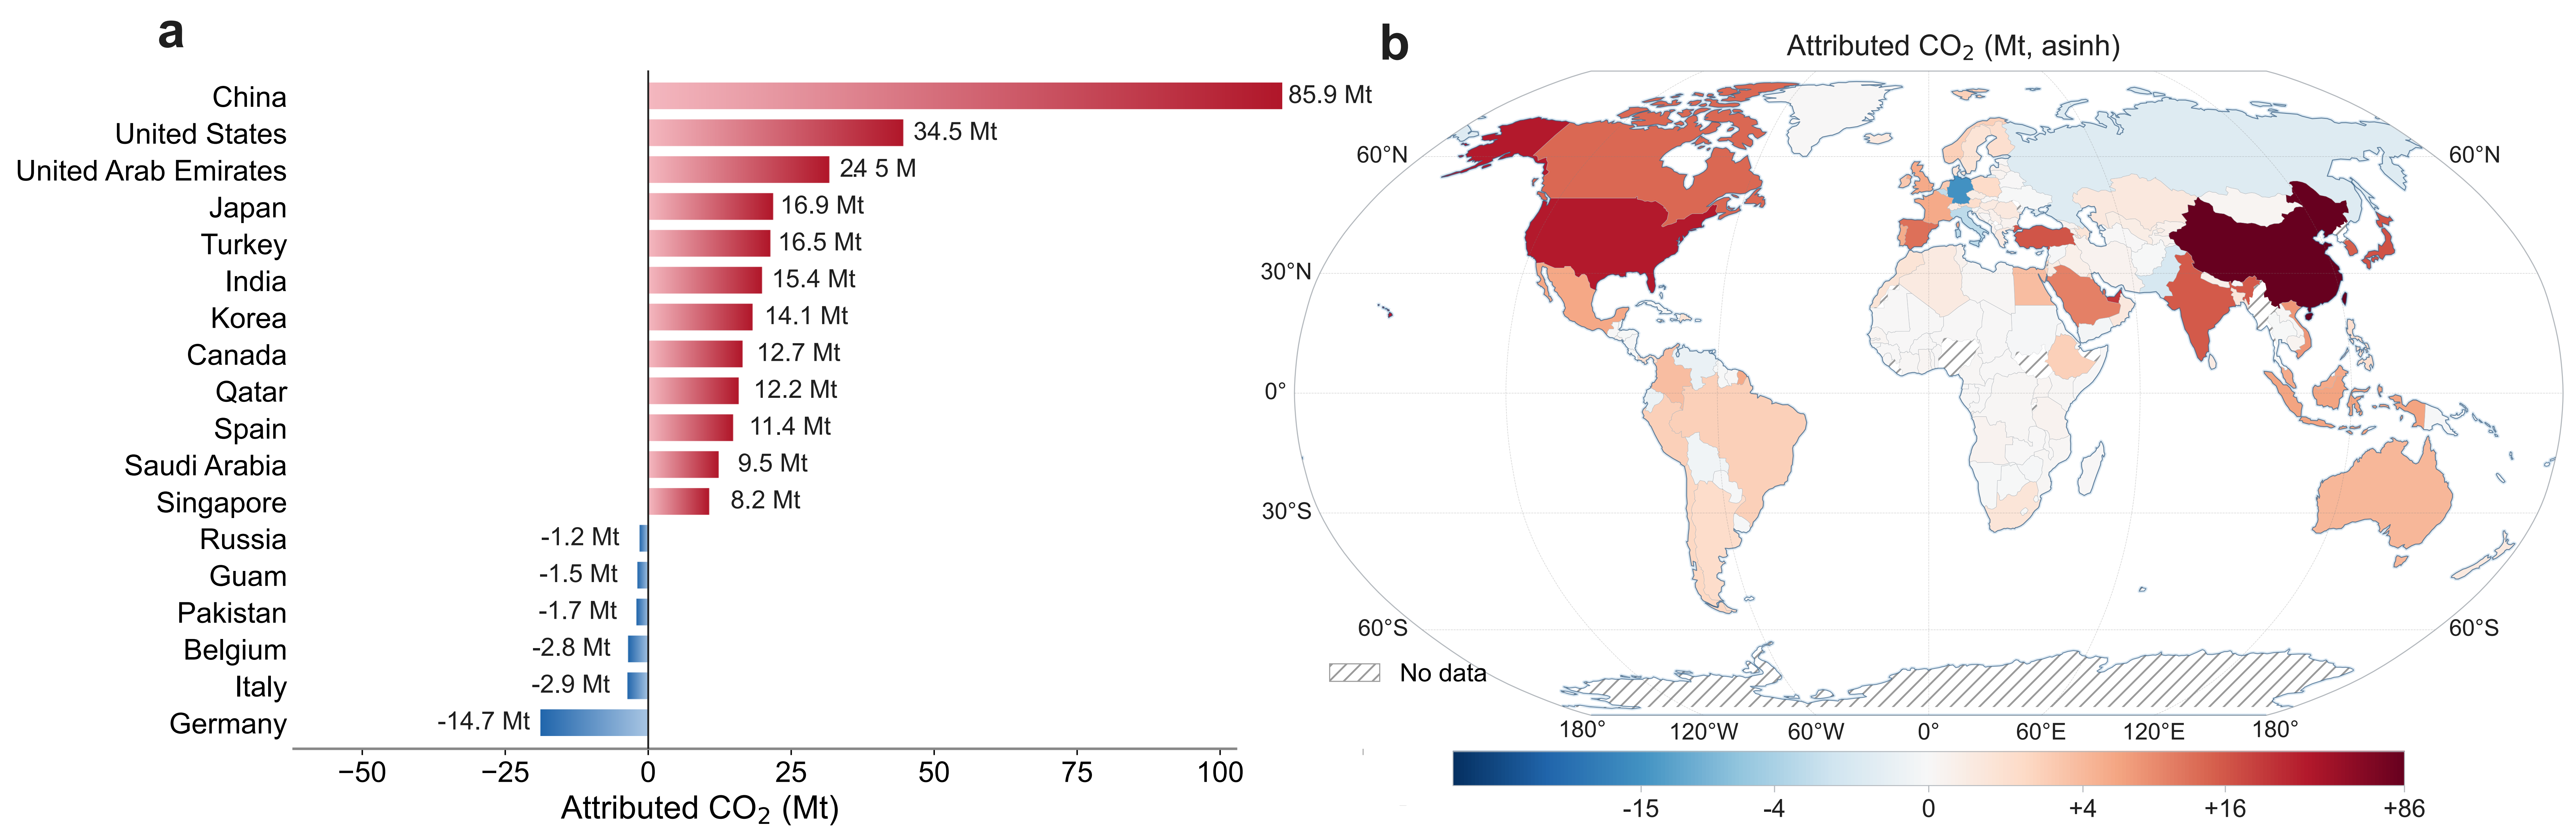
\includegraphics[width=0.98\textwidth]{Figure2_ab.png}
\caption{\textbf{Aviation CO$_2$ attributed to connectivity growth since 1996.} \textbf{a}, Aviation CO$_2$ in 2023 attributed to 1996--2023 connectivity growth, for the twelve largest positive countries and all countries below $-1$ Mt. \textbf{b}, The same attribution for every country (Mt, arcsinh colour scale; white denotes zero and hatching no data). The attribution applies the Feyrer-instrument elasticity to each country's connectivity change over its observed span; the world total is 348.7 Mt, 41.1\% of 2023 aviation CO$_2$, and its social cost is reported in Extended Data Table~\ref{tab:scc}.}
\label{fig:attrib}
\end{figure}

\subsection*{Fuel switching reverses emissions growth and yields net climate benefits}
Finally, we project world aviation CO$_2$ to 2050 under continued connectivity growth and sustainable aviation fuel (SAF) mandates (Fig.~\ref{fig:saf}). The preceding results show why fuel switching matters: additional flights drive the emissions response to connectivity, while efficiency improvements offset only 6\% of the increase. We combine our fuel-demand projection with fuel pathways from the Aviation Integrated Model (AIM), which limit SAF uptake by the pace of production growth and available feedstocks \citep{dray2019aim2015,dray2022}. Here, SAF comprises drop-in biofuels produced from biomass, wastes and residues, and power-to-liquid fuels synthesized from captured CO$_2$ and hydrogen.

Without fuel switching, well-to-wake emissions reach 1,777~Mt in 2050, 1.8 times the 2023 level of 986~Mt (848~Mt of direct combustion emissions plus upstream fuel-supply emissions), compared with 1,411~Mt under a low-growth case (Fig.~\ref{fig:saf}a,b). The clearest legislated trajectory to 2050 is ReFuelEU, which raises the SAF blending requirement from 2\% in 2025 to 70\% in 2050 (Regulation (EU) 2023/2405) but applies only at EU airports, which account for 16\% of world aviation fuel in our inventory. With airports elsewhere continuing to use fossil jet fuel, this mandate lowers global emissions in 2050 by 11\% relative to the no-SAF projection, to 1,583~Mt. Applying the same milestones worldwide lowers emissions by 65\%, to 617~Mt, and returns them to the 2023 level by 2040. Two further global mandates, with blending paths drawn from AIM scenarios, show how the outcome changes with ambition: a 38\% requirement lowers emissions by 35\%, to 1,158~Mt, while a 100\% requirement lowers them by 95\%, to 84~Mt, below the 2023 level from 2035. Fuel switching can therefore reverse emissions growth, with the scale and timing of the reduction depending on both the depth and geographic reach of the mandate.

The emissions reductions come with higher fuel costs (Fig.~\ref{fig:saf}c,d). Across the three global mandates, cumulative additional fuel costs over 2024--2050 range from \$806 billion to \$1,538 billion, or 11.3\% to 21.6\% above the all-fossil fuel bill. Valued at the US EPA social cost of carbon (central estimate), avoided climate damages amount to 130\%--193\% of these additional costs. As the value of avoided CO$_2$ rises and the modelled average cost of SAF falls over time, cumulative climate benefits exceed additional fuel costs in all three global mandate scenarios under the EPA estimate. Under the Interagency Working Group (IWG) estimate (lower bound), avoided damages cover only 36\%--52\% of additional costs. Fuel switching can therefore yield benefits greater than its additional fuel costs, depending on the social cost of carbon used.


\begin{figure}[H]
\centering
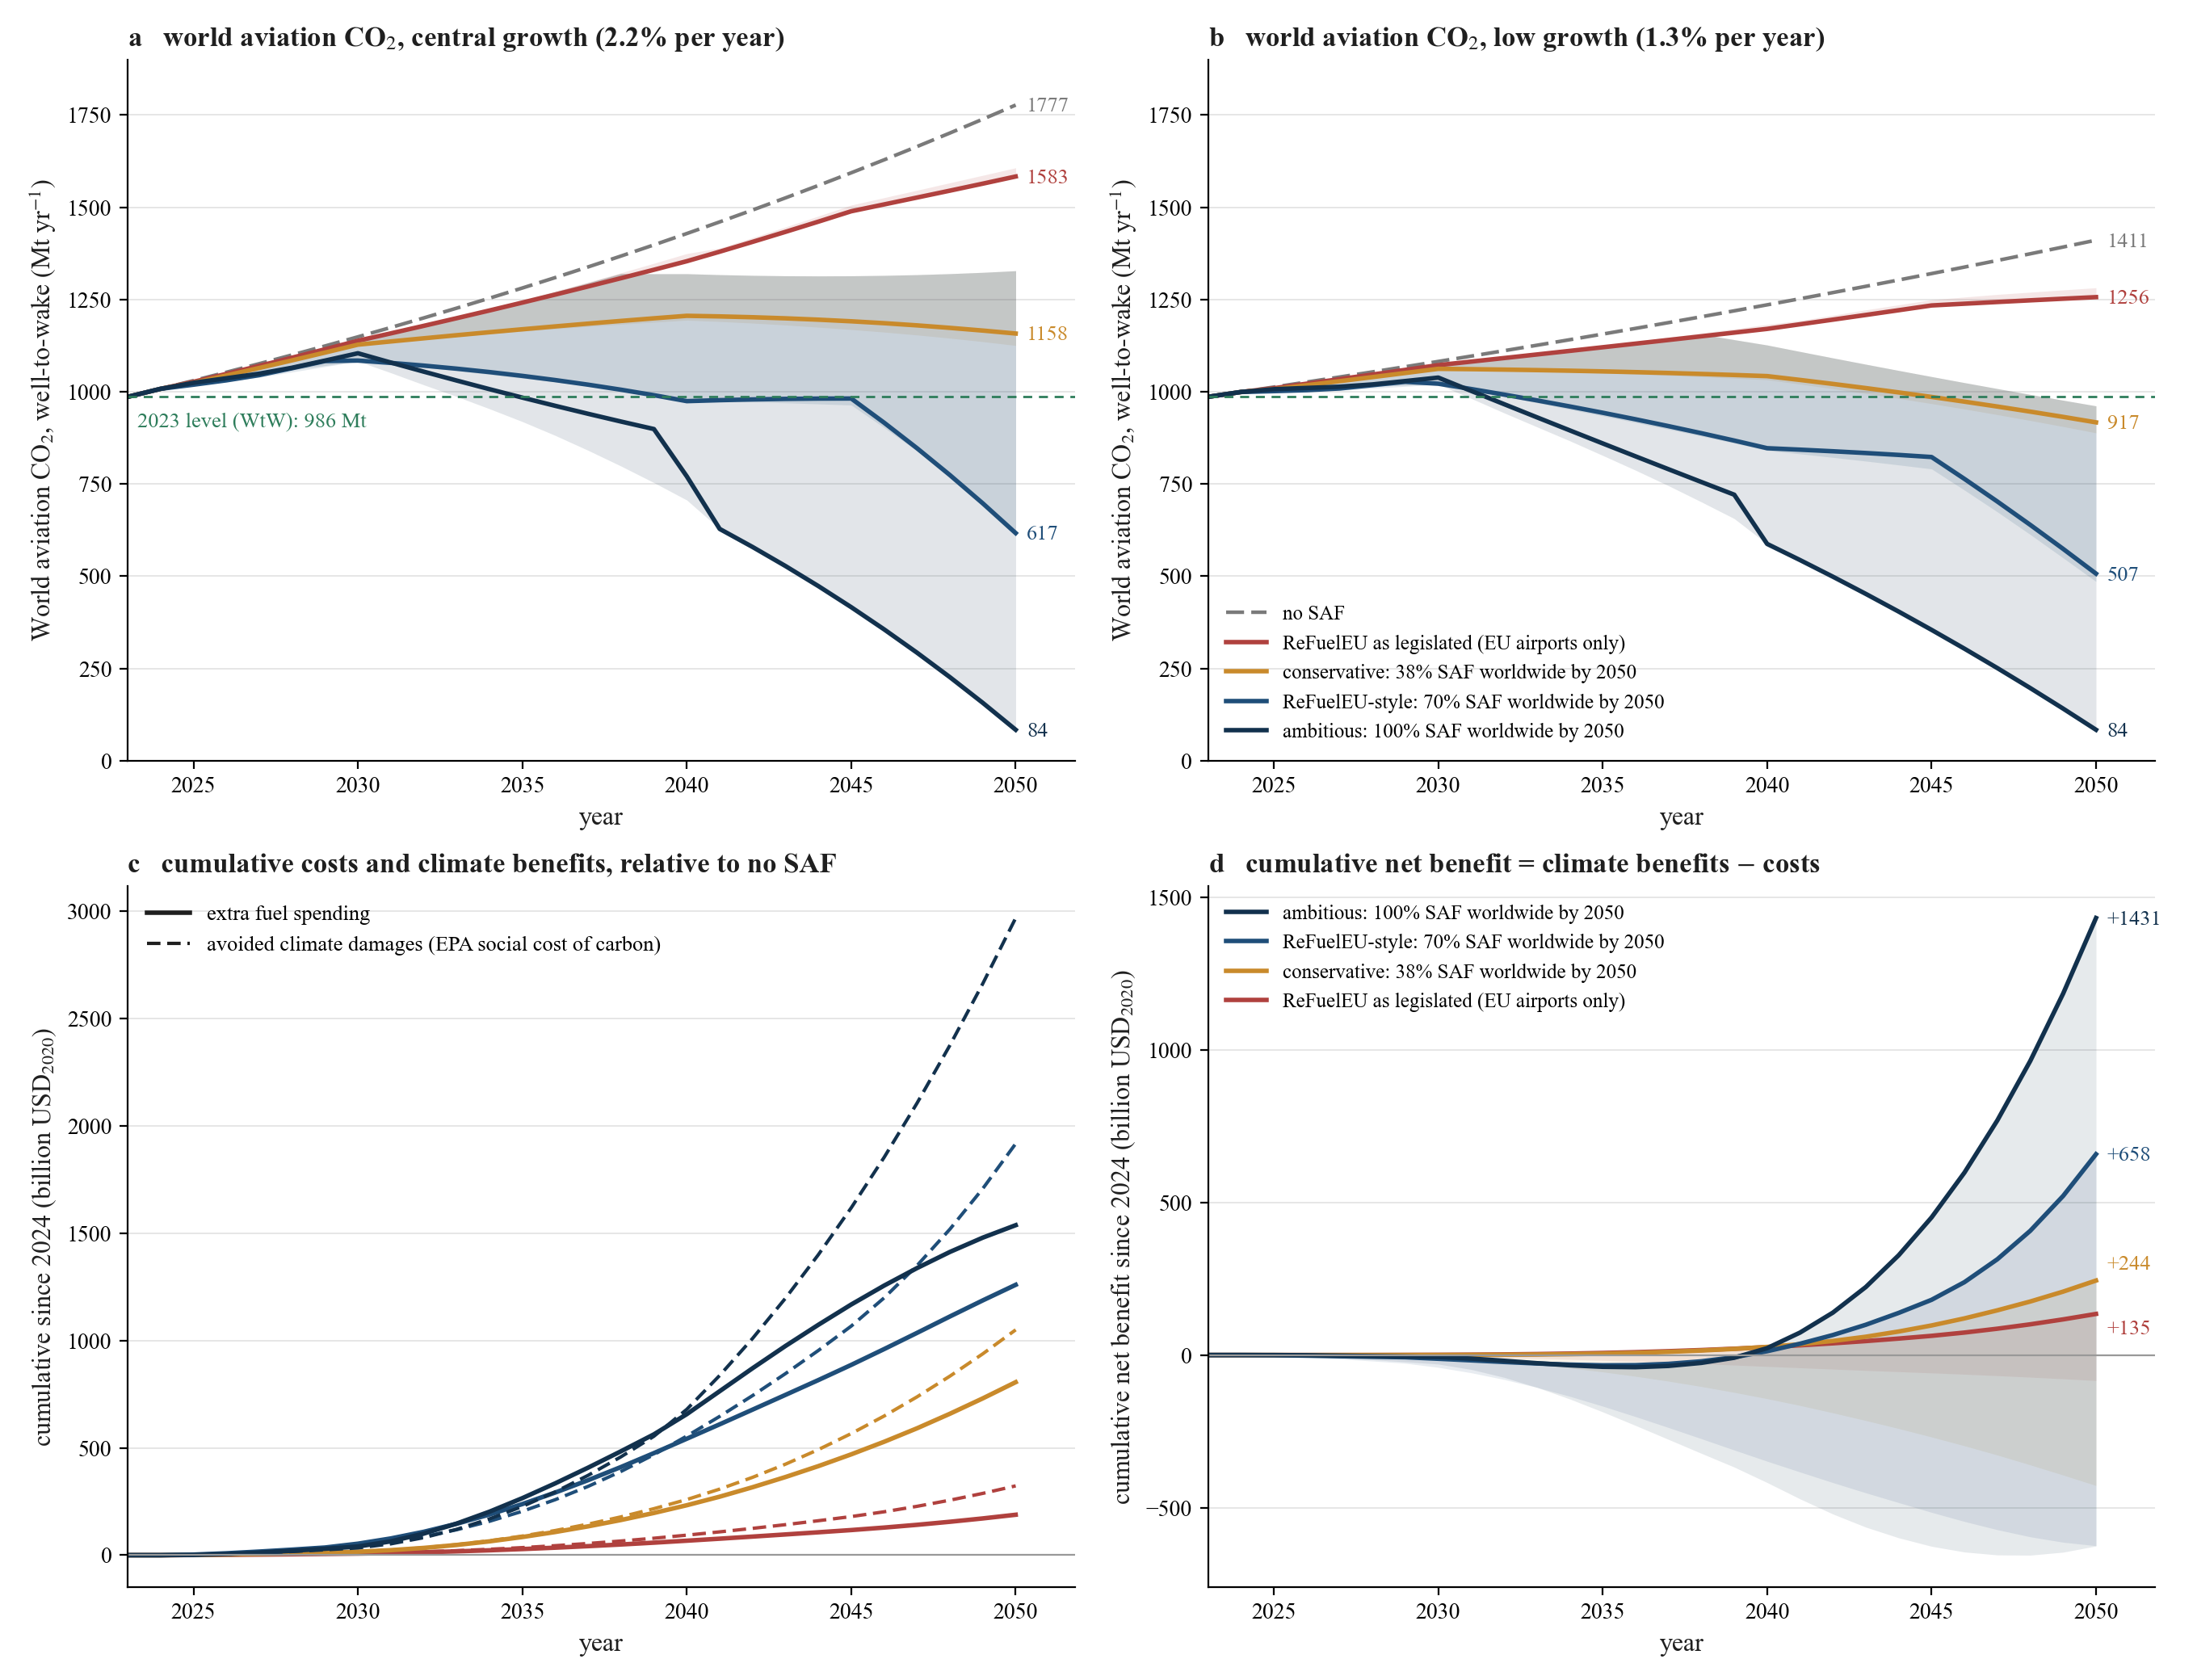
\includegraphics[width=0.98\textwidth]{CO2_SAF.png}
\caption{\textbf{World aviation CO$_2$ emissions, fuel costs and climate benefits under SAF mandates to 2050.} \textbf{a,b,} Well-to-wake CO$_2$ emissions under baseline connectivity growth (\textbf{a}, 2.2\% yr$^{-1}$) and low growth (\textbf{b}, 1.3\% yr$^{-1}$). The no-SAF path is compared with four mandates, with 2050 blending shares of 70\% at EU airports under ReFuelEU, 38\% worldwide, 70\% worldwide following the ReFuelEU milestones, and 100\% worldwide. Lines show mid-range fuel supply assumptions; shading spans pessimistic to optimistic assumptions about biomass availability and production capacity growth. The green dashed line marks 2023 emissions (986~Mt), and line-end labels show 2050 emissions in Mt. \textbf{c,} Cumulative additional fuel costs (solid) and the value of avoided CO$_2$ emissions using the US EPA social cost of carbon (dashed), relative to no SAF. \textbf{d,} Cumulative net benefits under the EPA estimate (central line), with shading extending to the lower estimates from Rennert et al.\ (2022) and the US Interagency Working Group (IWG).}
\label{fig:saf}
\end{figure}

%=======================================================================
\section*{Discussion}
%=======================================================================
Our results provide global causal evidence that air connectivity is a system-level driver of aviation CO$_2$, with effects that are strongest during network take-off and extend across national borders. Five implications follow. First, the emissions response to connectivity is carried primarily by additional flights. Because GACI combines network topology with service intensity, its elasticity captures system-level changes in network structure and supplied capacity rather than the addition of a single route. A one percent increase in GACI raises seat-kilometres by 5.64\% and CO$_2$ by 5.35\%. Changes in aircraft gauge, stage length and emissions intensity are not individually significant. The 0.29\% intensity decline offsets only 6\% of the scale response. Aviation decarbonization pathways often treat traffic growth as exogenous, whereas we identify network development as an important source \citep{bergero2023,dray2022}. Within the scenarios considered, sustained fuel switching materially lowers total emissions; the observed efficiency gains do not. Policy should therefore track absolute CO$_2$ and traffic growth and combine connectivity expansion with lower-carbon fuels, propulsion technologies and demand-side measures \citep{creutzig2018}.

Second, the global mean elasticity does not apply equally across countries. Identification is concentrated in the take-off stage of network development, and the response is largest in countries with low baseline connectivity. Continuous estimates suggest a declining, rather than vanishing, response. The economic gains from connectivity are also expected to be largest in weakly connected economies \citep{lenaerts2021,zhang2020,amico2026}, so marginal economic benefits and carbon consequences may be greatest in the same places. These results do not justify restricting access; they support coupling network expansion with early provision of lower-carbon fuels, cleaner aircraft and supporting infrastructure.

Third, connectivity creates effects across borders. A one percent increase in contiguous neighbours' connectivity raises own-country aviation CO$_2$ by about 2\%, mainly through international traffic. The effect follows land borders rather than a smooth distance gradient, indicating a regional network externality rather than a global spillover. It remains after accounting for neighbours' emissions and common regional shocks, which distinguishes it from the strategic interaction in emissions documented among neighbouring jurisdictions \citep{zhuwei2024}. The social-cost estimate is sizeable but depends on attribution and carbon valuation. This cross-border incidence matters for CORSIA, whose monitoring is based on reported international-flight emissions and whose offsetting obligations follow covered State pairs rather than the regional causal incidence of network expansion \citep{icao2018corsia}. National measures should therefore be complemented by regional coordination in airport investment, route development and low-carbon fuel supply.

Fourth, the airport results suggest where mitigation could be targeted. Eighty-five percent of attributed emissions is concentrated in the top 5\% of airports, with emerging hubs among the largest contributors. These descriptive estimates identify high-leverage sites for low-carbon fuel supply and infrastructure, not sole sources of causation or responsibility; the response extends across countries and routes.

Fifth, these implications should be interpreted in light of several limitations. Three direct diagnostics are consistent with the exclusion restriction (Methods), but identification is concentrated in the network-expansion era and in lower-connectivity countries. The later-period elasticity is identified only after excluding the COVID-19 collapse years \citep{lequere2020}; correlated global cycles and sectoral change remain possible channels. Emissions are schedule-based and do not reflect realized load factors. The airport attribution is descriptive; the country attribution and fuel-switching scenarios are partial-equilibrium calculations; and non-CO$_2$ climate effects, which account for a large part of aviation's warming, are excluded \citep{brazzola2022}. Policy assessments should therefore use development-stage-specific ranges rather than one global elasticity. Future work could separate GACI's topological and volumetric components and use route-level causal designs to test whether new links, centrality gains or traffic concentration drive changes in demand, schedules and fleet assignment. Coupling these pathways with deployment scenarios for sustainable aviation fuels, synthetic e-fuels and alternative propulsion systems could show when technological change offsets connectivity-induced growth in flights.

%=======================================================================
\section*{Methods}
%=======================================================================
\subsection*{Flight-level aviation CO$_2$ emissions}

We estimate CO$_2$ for every scheduled flight leg in the Official Airline Guide (OAG) schedules from January 1996 to June 2024, following the aviation chapter of the EMEP/EEA Air Pollutant Emission Inventory Guidebook \citep{eea2023} with engine-specific parameters from the ICAO Aircraft Engine Emissions Databank. Multi-stop services are split into their operated legs. Each leg's emissions are the sum of a landing-and-take-off (LTO) component below 3,000 feet and a climb--cruise--descent (CCD) component (Supplementary Note~2). OAG equipment codes are matched to the aircraft--engine configurations of the EEA database; where no exact type exists, the closest type in the same family is used. LTO emissions are computed for five modes (taxi-out, take-off, climb-out, approach and landing, taxi-in) as the standard time in mode (19, 0.7, 2.2, 4 and 7 minutes) times the engine fuel-flow rate, the number of engines and the fuel emission factor (3.15 kg CO$_2$ per kg of Jet A, 3.10 for aviation gasoline). CCD emissions interpolate the EEA aircraft-specific reference values linearly in flight distance, after converting the great-circle distance to the EEA flight distance following \citet{avogadro2024}. The inventory describes scheduled operations under standard conditions; it does not observe weather, routing or realized load factors.

\subsection*{Allocation of emissions to countries}

Country-year emissions require a rule for the en-route component of international flights. We keep departure- and arrival-side LTO emissions separate and assign them to the countries of the departure and arrival airports. The headline, departure-based (bunker) measure adds each flight's full CCD component to the departure country, mirroring the origin-side logic of international bunker accounting. Two alternatives bound this accounting choice: an LTO-only (territorial) measure that excludes CCD emissions, and a 50/50 measure that splits CCD emissions equally between the endpoint countries. The bunker and 50/50 measures coincide for domestic flights and preserve the same global total, so any difference between them reflects only the allocation of international en-route emissions (Supplementary Note~2). The elasticity is within 0.3 across the three rules (Extended Data Table~\ref{tab:alloc}).

\subsection*{Validation of the emissions inventory}

Against two independent global references, IATA industry statistics \citep{iata2018,iata2019,iata2024} and the OECD flight-level inventory \citep{clarke2022}, our world totals have weighted absolute percentage errors of 3.0\% (2004--2023) and 3.6\% (2013--2023); against carrier-reported fuel consumption from the U.S. Bureau of Transportation Statistics the error is 3.8\% over 1996--2023 (Extended Data Table~\ref{tab:validation_benchmarks}). The cross-country distribution matches the OECD territory-based series with a log-scale correlation of 0.999 over 2013--2018 (total variation distance 1.1\%) and 0.955 over 2019--2023, when the OECD series switches from schedules to realized ADS-B flights. LTO operations account for 12.4\% of CO$_2$, within the 10.8--13.5\% that \citet{quadros2022} report for the ICAO reference cycle. Supplementary Note~2 gives the details.

\subsection*{Global Air Connectivity Index}

We measure connectivity with the Global Air Connectivity Index (GACI) of \citet{cheung2020}, reconstructing the worldwide airport network for each year from OAG route-segment schedules, so that airports enter and leave the network as scheduled service begins or ceases. Airports are nodes, a link exists where scheduled service connects two airports, and its intensity $w_{ijt}=\sqrt{s_{it}s_{jt}/(d_{it}d_{jt})}$ combines the seat capacity $s$ and degree $d$ of the endpoints. GACI is the first principal component of five standardized indicators: degree, closeness and eigenvector centrality, which describe topology, and flow betweenness and regional importance, which add the intensity of connections (Supplementary Note~3). The loadings are positive and stable across years, the first component explains 63--77\% of the annual variation, and a pooled PCA correlates at 0.98 with the year-specific index. The headline national measure is the capacity-weighted mean of airport GACI over the airports $A_{ct}$ with scheduled service in country $c$ in year $t$,
\begin{equation}
\mathrm{GACI}^{\mathrm{cwm}}_{ct}
=
\frac{
\displaystyle
\sum_{i\in A_{ct}}
s_{it}\mathrm{GACI}_{it}
}{
\displaystyle
\sum_{i\in A_{ct}}
s_{it}
}.
\label{eq:nature_18}
\end{equation}
with the maximum, sum and unweighted mean as alternatives (Supplementary Note~3, equations~\ref{eq:nature_19}--\ref{eq:nature_21}). Because GACI responds to frequencies, capacity and partners' connectivity as well as to new routes, it captures both the extensive and the intensive margin of network development.

The estimation sample covers 182 countries over 1996--2023, comprising 4,634 country-year observations. Two of the 184 countries in the emissions panel are excluded: Cura\c{c}ao, for which the CERDI database records no sea distance, and New Caledonia, observed in a single year. Supplementary Table~\ref{tab:sumstat} reports summary statistics for all variables used in the analysis. Of the 6,356 airports represented in the emissions inventory, 5,354 are nodes in the connectivity network; airports not matched to the GACI network account for only 0.1\% of departure-based emissions, and airports that cannot be assigned to a country (0.02\% of emissions) are excluded from the country panel.

\subsection*{Estimation}
We estimate the effect of GACI on aviation CO$_2$ emissions based on the following equation:

\begin{equation}
\ln \mathrm{CO_2}_{ct} = \beta \,\ln \mathrm{GACI}_{ct}
 + \gamma \,\ln \mathrm{pop}_{ct} + \delta \,\ln \mathrm{seaMA}_{ct}
 + \alpha_c + \tau_t + \varepsilon_{ct},
\label{eq:main}
\end{equation}

where $\mathrm{CO_2}_{ct}$ denotes aviation CO$_2$ emissions and $\mathrm{GACI}_{ct}$ represents the GACI in country $c$ in year $t$. Among the GACI variants, we use $\mathrm{GACI}^{\mathrm{cwm}}_{ct}$ as our primary independent variable, while $\mathrm{GACI}^{\mathrm{max}}_{ct}$, $\mathrm{GACI}^{\mathrm{sum}}_{ct}$, and $\mathrm{GACI}^{\mathrm{mean}}_{ct}$ are used in supplementary analyses. $\mathrm{pop}_{ct}$ and $\mathrm{seaMA}_{ct}$ denote total population and sea market access (equation~\ref{eq:seama}), respectively, while $\alpha_c$ and $\tau_t$ represent country and year fixed effects, and $\varepsilon_{ct}$ is an idiosyncratic error term.

To address potential endogeneity concerns, we employ two-stage least squares (2SLS) estimation. The first-stage equation is specified as follows:

\begin{equation}
\ln \mathrm{GACI}_{ct} = \beta^{\mathrm{1st}} \,\mathrm{Z}_{ct}
 + \gamma^{\mathrm{1st}} \,\ln \mathrm{pop}_{ct} + \delta^{\mathrm{1st}} \,\ln \mathrm{seaMA}_{ct}
 + \alpha_c^{\mathrm{1st}} + \tau_t^{\mathrm{1st}} + \nu_{ct},
\label{eq:firststage}
\end{equation}

where $\mathrm{Z}_{ct}$ denotes the instrumental variable and $\nu_{ct}$ is the first-stage error term. The superscript ``$\mathrm{1st}$'' indicates parameters from the first-stage regression. Standard errors are clustered at the country level (182 clusters), and all first-stage statistics are cluster-robust. For comparison, heteroskedasticity-robust standard errors---which are approximately one-third the magnitude of the clustered standard errors---are reported in Supplementary Table~\ref{tab:exclusion2}. Furthermore, two-way clustering by country and year yields standard errors virtually identical to the baseline one-way country clustering.


\subsection*{Instruments and validity}

Time-varying country shocks, such as tourism booms or aviation deregulation, may expand air networks and raise emissions at the same time, and policy responses to rising emissions, such as slot restrictions or aviation taxes, may induce reverse causality. We therefore instrument connectivity with a shift-share instrument in the spirit of \citet{feyrer2019}, which uses the fact that the growth of aviation shortens the effective distance to foreign markets more for some countries than for others. For each country we compute air and sea market access as distance-weighted sums of foreign population,
\begin{equation}
\mathrm{airMA}_{ct}=\sum_{j\neq c}\frac{\mathrm{Pop}_{jt}}{d^{\,\mathrm{air}}_{cj}},
\qquad
\mathrm{seaMA}_{ct}=\sum_{j\neq c}\frac{\mathrm{Pop}_{jt}}{d^{\,\mathrm{sea}}_{cj}},
\label{eq:seama}
\end{equation}
where $\mathrm{Pop}_{jt}$ is the population of foreign country $j$ (World Bank World Development Indicators), $d^{\,\mathrm{air}}_{cj}$ is the great-circle distance in kilometres between the aviation centroids of $c$ and $j$, defined as the unweighted mean coordinates of each country's airports in the network, and $d^{\,\mathrm{sea}}_{cj}$ is the port-to-port sea distance from the CERDI-seadistance database \citep{bertoli2016}, which assigns landlocked countries the port of their transit country. Own-country population is excluded, the distance-decay exponent is one, and both sums run over the same set of partner countries. The instrument interacts a world aviation index with air market access fixed at its 1996 value,
\begin{equation}
Z_{ct}=a_t\times\ln \mathrm{airMA}_{c,1996},
\label{eq:feyrer}
\end{equation}
where $a_t$ is world scheduled seat capacity in year $t$, the sum of annual seat capacity over the airports of all countries in our panel in the OAG schedules (95 to 98\% of capacity in the global network, correlation 0.999 with the all-airport total), min--max scaled to $[0,1]$ over 1996--2023. Because $\mathrm{airMA}_{c,1996}$ is computed from 1996 populations, it is also defined for the 32 countries that join the network after 1996. Log sea market access, computed with contemporaneous populations, enters equations~\ref{eq:main} and \ref{eq:firststage} as a control, so that the instrument isolates the aviation-specific gain in market access rather than the general advantage of proximity to foreign populations, including the surface-shipping channel. The global aviation index and the 1996 geography are both external to a country's contemporaneous demand shocks and regulatory decisions.

The instrument is relevant: the first-stage Kleibergen--Paap $F$ is 18.4 (153.6 with heteroskedasticity-robust errors). Because any shifter of the form (global cycle $\times$ baseline characteristic) may proxy for size dynamics (global cycle $\times$ country size), we add interactions of the global cycle with baseline population, GDP and airport capacity to the first stage; on the 4,121 country-years of countries observed in 1996, the heteroskedasticity-robust $F$ falls only from 120.1 to 105.8.

The exclusion restriction requires that the instrument affect aviation CO$_2$ only through air connectivity, not through non-aviation channels. Three direct tests are consistent with it (Extended Data Table~\ref{tab:exclusion}, Panels A, C and D; Extended Data Fig.~\ref{fig:placebos}d). First, non-aviation emissions do not respond to the instrument: the reduced form on total territorial fossil CO$_2$ excluding domestic aviation is 0.05 (s.e.\ 0.12), against 0.68 (s.e.\ 0.15) for aviation CO$_2$, rejecting a general development channel that would raise all emissions. Second, the effect operates through air geography rather than geography in general: when the aviation cycle is interacted with 1996 sea market access instead of air market access and both interactions are entered, the sea term has a reduced form of $-$0.19 (s.e.\ 0.26) while the air term retains 0.82 (s.e.\ 0.21). Third, where the instrument cannot move connectivity it does not move emissions: in the top tercile of baseline connectivity, where the first stage is absent ($F$ = 0.2), the reduced form on CO$_2$ is 0.09 (s.e.\ 0.19), against 1.97 and 0.41 in the lower terciles.

Further checks support these results (Extended Data Table~\ref{tab:exclusion} and Supplementary Table~\ref{tab:exclusion2}). Adding development controls keeps the elasticity between 4.4 and 4.7. Replacing world seat capacity with world flights, world seat-kilometres, the world sum of GACI or a fuel-efficiency index, or setting the distance-decay exponent of air market access to 0.5 or 1.5, gives elasticities of 5.2 to 5.8, and two-way clustering by country and year leaves the standard error unchanged. Two caveats remain. First, coal and cement CO$_2$ rise with the instrument (reduced forms of 0.90 and 0.67), indicating some recomposition of non-aviation emissions. Second, the aviation cycle is highly correlated with the world GDP and trade cycles (0.82 and 0.84), and entering either rival cycle interacted with the same geography removes the first stage (Extended Data Table~\ref{tab:exclusion}, Panel B). The instrument therefore cannot separate aviation growth from general world growth; the exclusion restriction rests on the air-market-access geography, and the placebo outcomes in Panel A show that this geography, interacted with the cycle, does not move total non-aviation emissions. Alternative constructions that avoid these caveats, such as the air-minus-sea advantage interacted with the cycle, give weak first stages ($F$ of 1.0 and 5.6).

Finally, an aviation-accident instrument, lagged fatal accidents and accident deaths from the Aviation Safety Network, is too weak to use on its own (first-stage $F$ of 1.1 to 4.2; 2SLS 5.6 with a standard error of 2.2 for lagged fatal accidents). Entered jointly with the Feyrer instrument it gives an elasticity of 5.1, and the Hansen test does not reject the overidentifying restriction ($p$ = 0.82 and 0.96; Supplementary Table~\ref{tab:accident_iv}).

\subsection*{Decomposition of the emissions elasticity}

National aviation CO$_2$ is the product of departing flights $F_{ct}$, seats per flight, kilometres per seat and CO$_2$ per seat-kilometre,
\begin{equation}
\mathrm{CO_2}_{ct} = F_{ct} \times \frac{S_{ct}}{F_{ct}} \times
\frac{K_{ct}}{S_{ct}} \times \frac{\mathrm{CO_2}_{ct}}{K_{ct}},
\label{eq:identity}
\end{equation}
where $S_{ct}$ and $K_{ct}$ are departing seats and seat-kilometres. Estimating the baseline 2SLS specification (equation~\ref{eq:main}) for the log of each component on the same sample gives an additive decomposition of the total elasticity,
\begin{equation}
\beta_{\mathrm{CO_2}} = \beta_{\mathrm{flights}} + \beta_{\mathrm{gauge}} +
\beta_{\mathrm{stage}} + \beta_{\mathrm{intensity}},
\label{eq:decomp}
\end{equation}
in which the first three terms sum to the seat-kilometre elasticity. A constant load factor scales scheduled capacity by a constant and is absorbed by the fixed effects. We apply the decomposition to all departures, to international and domestic departures separately, and within baseline income and connectivity terciles.

\subsection*{Spatial econometric specifications and spillover effects}

To test for cross-border spillovers we extend equation~\ref{eq:main} to the general spatial model
\begin{equation}
\ln \mathrm{CO_2}_{ct} = \rho \, W \ln \mathrm{CO_2}_{ct} + \beta \,\ln \mathrm{GACI}_{ct} + \theta \, W \ln \mathrm{GACI}_{ct}
 + \gamma \,\ln \mathrm{pop}_{ct} + \delta \,\ln \mathrm{seaMA}_{ct} + \alpha_c + \tau_t + u_{ct},
\label{eq:spatial_general}
\end{equation}
\begin{equation}
u_{ct} = \lambda \, W u_{ct} + \varepsilon_{ct},
\label{eq:spatial_error}
\end{equation}
where $W$ is a spatial weight matrix. Zero restrictions on $(\rho,\theta,\lambda)$ give the SLX ($\rho=\lambda=0$), SAR ($\theta=\lambda=0$), SEM ($\rho=\theta=0$), SDM ($\lambda=0$) and SDEM ($\rho=0$) models. $W$ is a row-normalized land-contiguity matrix from Natural Earth boundaries, applied within each year so that the stacked matrix is block-diagonal; the 38 countries without a land neighbour have a zero row, and an indicator absorbs this structural zero. Alternative weights (five nearest countries, distance bands, exponential kernels, regional leave-out means and inverse distance) are reported in Extended Data Tables~\ref{tab:spillover}, \ref{tab:spill_ext} and \ref{tab:spatial_ext}.

Panel A of Table~\ref{tab:spatial} estimates the models on the within-transformed data by OLS (SLX) or maximum likelihood, summing the log-determinant over the yearly blocks. Panel B follows the generalized spatial two-stage least squares approach of \citet{kelejian1998}: own connectivity is instrumented by the Feyrer shifter $Z_{ct}$ and neighbours' connectivity by its identically weighted average $WZ_{ct}$; the spatial lag of the outcome is instrumented with the first and second spatial lags of the shifter and the exogenous controls; and in the error models $\lambda$ is obtained by a moments estimator from the 2SLS residuals before the equation is re-estimated on the spatially filtered variables. Direct, indirect and total effects are the yearly-block averages of the diagonal, the off-diagonal row sums and the row sums of $(I-\rho W)^{-1}(\beta I + \theta W)$, with standard errors from 100 draws of the coefficient vector. Standard errors are clustered by country.

Because the joint first stage is weak under country clustering (Kleibergen--Paap $F$ of 3.3 for contiguity, with Sanderson--Windmeijer conditional $F$ of 6.7 for own and 13.0 for neighbour connectivity), we also report Anderson--Rubin confidence sets for the neighbour coefficient, obtained by inverting the cluster-robust test over a grid of null values; for contiguity the 95\% set is [0.2, 3.0] and excludes zero (Extended Data Table~\ref{tab:spillover}). A permutation placebo reassigns countries at random in the weight matrix, rebuilds the spatial exposures and re-estimates the specification 500 times; its $p$-value is the share of draws whose absolute $t$-statistic on the neighbour term exceeds the actual one.

\subsection*{Mediation analysis}

We also ask how much of the effect runs through flight frequency, seat-kilometres and the international share of traffic, one mediator at a time (Extended Data Table~\ref{tab:mediation}). An instrumental-variable decomposition instruments log GACI with the Feyrer shifter in both the mediator and the outcome equation and combines the two paths by the product method, with delta-method (Sobel) standard errors. The algorithm of \citet{imai2010} uses quasi-Bayesian simulation on least-squares models with country and year fixed effects. The mediators overlap, so their shares are not mutually exclusive and do not sum to 100\%.

\subsection*{Attribution and fuel-switching scenarios}
The share of 2023 emissions attributed to post-1996 connectivity growth is
$1 - \exp(-\beta\,\Delta \ln \mathrm{GACI}_c)$, applied to 2023 levels;
because $\beta$ far exceeds one, country-level shares are extreme for
fast-growing countries and the world total (41.1\%) is the more
conservative summary. The attribution covers all 184 countries in the emissions panel; for the 34 countries entering the panel after 1996 and the 18 whose series end before 2023, the change is taken between the first and last observed years. The airport-level attribution applies the same
formula to each airport's change in log GACI between 1996, or its first
year in the network, and 2023; its sum (346 Mt) is close to the country
total because the elasticity is applied to the same emissions base. We then rank airports by attributed emissions and compare the cumulative shares held by the top 1, 5, 10 and 25\% of airports with their shares of actual 2023 emissions (Extended Data Table~\ref{tab:airport_conc} and Extended Data Fig.~\ref{fig:ed_temporal_airport}b,c).

For the fuel-switching scenarios, we project world fuel demand from the
2023 inventory as
\begin{equation}
F_t=F_{2023}\exp[\beta_m g(t-2023)],
\end{equation}
where $F_{2023}=11.6$~EJ, $\beta_m=2.948$ is the estimated
mature-network elasticity (Extended Data Table~\ref{tab:temporal},
Panel~C), and $g$ is the average annual change in log connectivity
across countries over 2010--2019. We set $g=0.0074$ in the central
case and $g=0.0045$ in the low-growth case. Because $\beta_m$ is a
reduced-form emissions elasticity that already captures the observed
efficiency response, we apply no separate emissions-intensity trend.

We compare four blending paths: (1) ReFuelEU at EU airports, with mandated shares rising from 2\% in 2025 to 70\% in 2050; (2) the same ReFuelEU milestones applied worldwide; and (3) two global paths reaching 38\% and 100\% in 2050, respectively. The latter two paths follow schedules distributed with the Aviation Integrated Model (AIM) \citep{dray2022}. We interpolate linearly between milestones.

Alternative-fuel use in each path is limited by the required blending share, production-capacity growth and available feedstocks. We use pathway-specific supply assumptions, well-to-wake CO$_2$ intensities, and levelized costs from the AIM fuel inputs \citep{dray2019aim2015,dray2022}. Biofuels are allocated across available pathways in order of feedstock cost, while power-to-liquid fuel can supply any remaining required volume subject to its own capacity limit. We calculate annual well-to-wake CO$_2$ emissions as
\begin{equation}
E_t=(F_t-Q_t)I_{\mathrm{fossil}}+\sum_p Q_{pt}I_{pt},
\end{equation}
where $Q_{pt}$ is the fuel energy supplied by alternative pathway $p$, $Q_t=\sum_p Q_{pt}$, and $I_{\mathrm{fossil}}$ and $I_{pt}$ are the corresponding well-to-wake CO$_2$ intensities. The lines in Fig.~\ref{fig:saf}a,b use the same central supply assumptions across all four paths; the shaded ranges reflect pessimistic and optimistic assumptions about biomass availability and production-capacity growth.

We estimate the additional fuel cost of each path as $\sum_p Q_{pt}(c_{pt}-p_t)$, where $c_{pt}$ and $p_t$ are the costs per unit of fuel energy for alternative pathway $p$ and fossil jet fuel, respectively. Fuel-cost assumptions follow \citet{dray2022}. We value CO$_2$ using three social-cost-of-carbon (SCC) estimates: \$51 per tonne from the US Interagency Working Group at a 3\% discount rate \citep{iwg2021}, \$185 from \citet{rennert2022} at a 2\% near-term discount rate, and approximately \$190 from the US Environmental Protection Agency (EPA) under its 2\% Ramsey approach \citep{epa2023}. For the fuel-switching paths, we use each source's SCC for the year of emission. Figure~\ref{fig:saf}d shows the EPA schedule as the upper bound and the Rennert and IWG schedules as lower-valued comparisons. We express both additional fuel costs and monetized CO$_2$ benefits in constant 2020 US dollars, and discount annual costs and benefits over 2024--2050 to 2023.

\subsection*{Data availability}
The OAG schedule data are proprietary and were used under licence; they cannot be redistributed. The country-year panel used in the regressions (aviation CO$_2$ under the three allocation rules, connectivity, instrument, controls and placebo outcomes), the airport-year GACI panel and the attribution and scenario outputs will be deposited in a public repository on publication. The benchmark and control series are available from the cited sources: IATA and OECD emissions statistics, the U.S. Bureau of Transportation Statistics, the World Development Indicators, the CERDI-seadistance database, the Global Carbon Project via Our World in Data, EDGAR and the Aviation Safety Network.

\subsection*{Code availability}
The Python code that builds the emissions inventory, the connectivity network and the instruments, and the Stata code that produces all tables and figures, will be deposited with the data on publication.

%=======================================================================
% Extended Data and Supplementary displays
% At submission these move to the Extended Data template; numbering below
% is by order of citation in the main text.
%=======================================================================
\clearpage
\section*{Extended Data}
\setcounter{table}{0}\setcounter{figure}{0}
\renewcommand{\tablename}{Extended Data Table}
\renewcommand{\figurename}{Extended Data Fig.}

\begin{table}[H]
\centering
\adjustbox{max width=\textwidth, max totalheight=0.9\textheight}{%
\begin{threeparttable}
\caption{Allocation of emissions to countries: bunker, territorial (LTO) and 50/50 rules}
\label{tab:alloc}
\footnotesize
\begin{tabular}{lccc}
\toprule
 & Bunker CO$_2$ & LTO CO$_2$ & 50/50 CO$_2$ \\
 & (1) & (2) & (3) \\
\midrule
\multicolumn{4}{l}{\textit{Panel A. OLS}} \\
  ln GACI (cwm) & 3.388$^{***}$ & 2.916$^{***}$ & 3.365$^{***}$ \\
   & (0.364) & (0.366) & (0.362) \\
  $N$ & 4,634 & 4,634 & 4,634 \\
\midrule
\multicolumn{4}{l}{\textit{Panel B. 2SLS, Feyrer instrument, capacity-weighted mean}} \\
  ln GACI (cwm) & 5.347$^{***}$ & 5.701$^{***}$ & 5.300$^{***}$ \\
   & (1.076) & (1.182) & (1.069) \\
  KP $F$ & 18.4 & 18.4 & 18.4 \\
  $N$ & 4,634 & 4,634 & 4,634 \\
\midrule
\multicolumn{4}{l}{\textit{Panel C. 2SLS, GACI sum}} \\
  ln GACI (sum) & 2.153$^{***}$ & 2.296$^{***}$ & 2.134$^{***}$ \\
   & (0.524) & (0.502) & (0.517) \\
  KP $F$ & 14.0 & 14.0 & 14.0 \\
  $N$ & 4,634 & 4,634 & 4,634 \\
\midrule
\multicolumn{4}{l}{\textit{Panel D. 2SLS, GACI max}} \\
  ln GACI (max) & 4.548$^{***}$ & 4.850$^{***}$ & 4.508$^{***}$ \\
   & (0.841) & (0.899) & (0.835) \\
  KP $F$ & 21.0 & 21.0 & 21.0 \\
  $N$ & 4,634 & 4,634 & 4,634 \\
\midrule
\multicolumn{4}{l}{\textit{Panel E. 2SLS, GACI mean}} \\
  ln GACI (mean) & 5.562$^{***}$ & 5.931$^{***}$ & 5.514$^{***}$ \\
   & (1.389) & (1.465) & (1.384) \\
  KP $F$ & 29.3 & 29.3 & 29.3 \\
  $N$ & 4,634 & 4,634 & 4,634 \\
\bottomrule
\end{tabular}
\begin{tablenotes}[flushleft]
\footnotesize
\item Notes: Specifications as in Table~\ref{tab:main}. Column (1) repeats the headline bunker measure (all cruise plus departure-side LTO assigned to the departure country); column (2) uses landing-and-take-off emissions only (territorial rule); column (3) splits cruise emissions equally between the endpoint countries. The three rules give elasticities within 0.3 of one another under every aggregation of airport connectivity. Standard errors clustered by country in parentheses; the Kleibergen--Paap $F$ is cluster-robust. $^{***}$, $^{**}$, $^{*}$: significance at 1, 5, and 10\%.
\end{tablenotes}
\end{threeparttable}}
\end{table}

\begin{table}[H]
\centering
\adjustbox{max width=\textwidth, max totalheight=0.9\textheight}{%
\begin{threeparttable}
\caption{Exclusion-restriction diagnostics for the Feyrer instrument}
\label{tab:exclusion}
\scriptsize
\begin{tabular}{lcccc}
\toprule
 & Reduced form & 2SLS & KP $F$ & $N$ \\
\midrule
\multicolumn{5}{l}{\textit{Panel A. Outcomes: coefficient on the instrument (reduced form) and on log GACI (2SLS)}} \\
  Aviation CO$_2$ (total, our series) & 0.685$^{***}$ (0.149) & 5.35$^{***}$ (1.08) & 18.4 & 4,634 \\
  Aviation CO$_2$ (international) & 0.665$^{***}$ (0.148) & 5.19$^{***}$ (1.04) & 18.4 & 4,634 \\
  Territorial fossil CO$_2$ excl.\ domestic aviation (GCP/OWID) & 0.049 (0.120) & 0.39 (0.95) & 17.1 & 4,576 \\
  Oil CO$_2$ excl.\ domestic aviation (OWID) & -0.115 (0.110) & -0.91 (0.89) & 17.1 & 4,576 \\
  Transport CO$_2$ excl.\ domestic aviation (EDGAR) & 0.111 (0.117) & 0.90 (0.94) & 15.8 & 4,461 \\
  Power industry CO$_2$ (EDGAR) & -0.365 (0.288) & -2.96 (2.51) & 15.3 & 4,409 \\
  Buildings CO$_2$ (EDGAR) & -0.140 (0.153) & -1.13 (1.23) & 15.8 & 4,460 \\
  Industrial combustion CO$_2$ (EDGAR) & 0.182 (0.168) & 1.53 (1.48) & 14.6 & 4,432 \\
  Coal CO$_2$ (OWID) & 0.896$^{***}$ (0.314) & 15.72 (10.06) & 2.5 & 3,030 \\
  Gas CO$_2$ (OWID) & -0.333 (0.316) & -4.28 (4.98) & 3.7 & 2,863 \\
  Cement CO$_2$ (OWID) & 0.665$^{***}$ (0.232) & 6.07$^{**}$ (2.70) & 8.9 & 3,476 \\
  Agriculture CO$_2$ (EDGAR) & -0.421$^{*}$ (0.221) & -4.06 (2.74) & 6.5 & 2,667 \\
\midrule
\multicolumn{5}{l}{\textit{Panel B. Content of the global cycle: first stage of the aviation-technology instrument with rival cycle $\times$ geography added}} \\
 & First-stage $\pi$ & 2SLS & Partial $F$ & $N$ \\
  Aviation technology $\times$ air geography (baseline) & 0.128$^{***}$ (0.030) & 5.35$^{***}$ (1.08) & 18.4 & 4,634 \\
  \quad plus oil price $\times$ geography & 0.103$^{***}$ (0.027) & 4.84$^{***}$ (1.15) & 14.7 & 4,634 \\
  \quad plus world GDP $\times$ geography & 0.011 (0.028) & -2.64 (11.92) & 0.2 & 4,634 \\
  \quad plus world exports $\times$ geography & -0.005 (0.028) & 28.44 (162.69) & 0.0 & 4,634 \\
  \quad plus all three & -0.013 (0.026) & 13.30 (25.58) & 0.2 & 4,634 \\
  World GDP $\times$ geography alone & 0.170$^{***}$ (0.037) & RF 0.950$^{***}$ (0.197) & 21.4 & 4,634 \\
  Oil price $\times$ geography alone & 0.103$^{***}$ (0.023) & RF 0.631$^{***}$ (0.128) & 20.0 & 4,634 \\
  World exports $\times$ geography alone & 0.169$^{***}$ (0.036) & RF 0.947$^{***}$ (0.195) & 21.9 & 4,634 \\
\midrule
\multicolumn{5}{l}{\textit{Panel C. Placebo instrument: aviation technology $\times$ 1996 sea market access}} \\
 & First-stage $\pi$ & Reduced form & Partial $F$ & $N$ \\
  Sea-geography instrument alone & 0.117$^{***}$ (0.033) & 0.482$^{***}$ (0.171) & 12.6 & 4,634 \\
  Sea-geography instrument, air-geography instrument included & 0.033 (0.051) & -0.187 (0.257) & 0.4 & 4,634 \\
  Air-geography instrument, sea-geography instrument included & 0.104$^{**}$ (0.044) & 0.824$^{***}$ (0.213) & 5.6 & 4,634 \\
  \quad 2SLS with the sea interaction as a control & \multicolumn{2}{c}{7.95$^{***}$ (2.90)} & 5.6 & 4,634 \\
\midrule
\multicolumn{5}{l}{\textit{Panel D. Zero-first-stage test by baseline connectivity tercile}} \\
 & First-stage $\pi$ & Reduced form (CO$_2$) & Partial $F$ & $N$ \\
  Low baseline connectivity & 0.263$^{***}$ (0.065) & 1.966$^{***}$ (0.351) & 16.4 & 1,453 \\
  Middle & 0.081$^{*}$ (0.042) & 0.410$^{*}$ (0.228) & 3.7 & 1,526 \\
  High (instrument does not move GACI) & 0.024 (0.052) & 0.095 (0.186) & 0.2 & 1,655 \\
\midrule
\multicolumn{5}{l}{\textit{Panel E. Development-channel controls added sequentially (2SLS coefficient on log GACI)}} \\
 & 2SLS & & KP $F$ & $N$ \\
  Baseline (log population, log sea market access) & 5.35$^{***}$ (1.08) & & 18.4 & 4,634 \\
  \quad plus log GDP & 4.45$^{***}$ (1.13) & & 11.8 & 4,634 \\
  \quad plus trade/GDP & 4.45$^{***}$ (1.40) & & 8.9 & 4,602 \\
  \quad plus urban share & 4.38$^{***}$ (1.38) & & 9.6 & 4,602 \\
  \quad plus FDI/GDP & 4.57$^{***}$ (1.27) & & 11.1 & 4,416 \\
  \quad plus log tourist arrivals & 4.72$^{***}$ (1.50) & & 8.9 & 3,444 \\
  Baseline on the common sample of the last row & 5.69$^{***}$ (1.32) & & 16.9 & 3,444 \\
\bottomrule
\end{tabular}
\begin{tablenotes}\scriptsize
\item All regressions include country and year fixed effects, log population and log sea market access; standard errors clustered by country in parentheses. Panel A: reduced form of each log outcome on the Feyrer interaction; non-aviation series are Global Carbon Project territorial CO$_2$ (via Our World in Data; domestic aviation subtracted) and EDGAR v2024 sectoral CO$_2$. Panel B: rival cycles are world real GDP, the Brent price and world real exports, min-max scaled and interacted with log 1996 air market access (correlations with the aviation index 0.82, 0.53 and 0.84). Panel C replaces air by sea market access in the interaction. Panel D: terciles of 1996 capacity-weighted GACI. Panel E: controls from the World Bank World Development Indicators; Venezuela's trade share for 1996--2011, reported as zero, is treated as missing. $^{***}$ $p<0.01$, $^{**}$ $p<0.05$, $^{*}$ $p<0.1$.
\end{tablenotes}
\end{threeparttable}}
\end{table}

\begin{table}[H]
\centering
\adjustbox{max width=\textwidth, max totalheight=0.9\textheight}{%
\begin{threeparttable}
\caption{Temporal split of the connectivity elasticity}
\label{tab:temporal}
\footnotesize
\begin{tabular}{lcccc}
\toprule
 & \multicolumn{1}{c}{Bunker CO$_2$} & \multicolumn{1}{c}{Intl.\ CO$_2$} & \multicolumn{1}{c}{Seat-km} & \multicolumn{1}{c}{Intensity} \\
 & (1) & (2) & (3) & (4) \\
\midrule
\multicolumn{5}{l}{\textit{Panel A. Full sample, 1996--2023}} \\
  ln GACI (cwm) & 5.347$^{***}$ & 5.192$^{***}$ & 5.641$^{***}$ & -0.294 \\
   & (1.076) & (1.043) & (1.194) & (0.286) \\
  KP $F$ & 18.4 & 18.4 & 18.4 & 18.4 \\
  $N$ & 4,634 & 4,634 & 4,634 & 4,634 \\
\midrule
\multicolumn{5}{l}{\textit{Panel B. Network-expansion era, 1996--2007}} \\
  ln GACI (cwm) & 5.609$^{***}$ & 5.578$^{***}$ & 4.754$^{***}$ & 0.854$^{**}$ \\
   & (1.092) & (1.082) & (0.993) & (0.371) \\
  KP $F$ & 25.4 & 25.4 & 25.4 & 25.4 \\
  $N$ & 1,883 & 1,883 & 1,883 & 1,883 \\
\midrule
\multicolumn{5}{l}{\textit{Panel C. Mature-network era, 2010--2023 (excl.\ 2020--2021)}} \\
  ln GACI (cwm) & 2.948$^{**}$ & 2.904$^{***}$ & 3.862$^{***}$ & -0.914$^{*}$ \\
   & (1.199) & (1.095) & (1.199) & (0.494) \\
  KP $F$ & 10.7 & 10.7 & 10.7 & 10.7 \\
  $N$ & 2,065 & 2,065 & 2,065 & 2,065 \\
\bottomrule
\end{tabular}
\begin{tablenotes}[flushleft]
\footnotesize
\item Notes: 2SLS with the Feyrer instrument; specifications as in Table~\ref{tab:main}. Panels B and C split the sample at its midpoint (2010) and exclude the crisis years: Panel B ends before the global financial crisis (2008--2009) and Panel C drops the COVID-19 collapse (2020--2021). The unrestricted 2010--2023 split (not shown) has a weak first stage (KP $F$ = 3.2), driven by the COVID years, whose exclusion in Panel C restores $F$ to 10.7; its estimates appear in grey in Extended Data Fig.~\ref{fig:ed_temporal_airport}a. Standard errors clustered by country in parentheses; Kleibergen--Paap $F$ statistics are cluster-robust. $^{***}$, $^{**}$, $^{*}$: significance at 1, 5, and 10\%.
\end{tablenotes}
\end{threeparttable}}
\end{table}

\begin{table}[H]
\centering
\adjustbox{max width=\textwidth, max totalheight=0.9\textheight}{%
\begin{threeparttable}
\caption{Causal mediation of the connectivity effect on aviation CO$_2$}
\label{tab:mediation}
\footnotesize
\begin{tabular}{lccccc}
\toprule
\multicolumn{6}{l}{\textit{Panel A. Instrumental-variable product of coefficients (2SLS scale; total effect 5.347)}} \\
Mediator & $a$: GACI$\rightarrow M$ & $b$: $M\rightarrow$CO$_2$ & ACME ($a\times b$) & Sobel $p$ & Share mediated \\
\midrule
  Flight frequency & 6.760 & 0.667 & 4.508 & 0.000 & 84.3\% \\
  Seat-kilometres & 5.641 & 0.801 & 4.521 & 0.000 & 84.5\% \\
  International share & 0.019 & -1.605 & -0.031 & 0.868 & -0.6\% \\
\midrule
\multicolumn{6}{l}{\textit{Panel B. Imai, Keele and Yamamoto (2010) mediation (OLS scale; total effect 3.582)}} \\
Mediator & ACME & Direct effect & Total effect & & Share mediated \\
\midrule
  Flight frequency & 1.766 & 1.816 & 3.582 & & 49.3\% \\
  Seat-kilometres & 3.424 & 0.159 & 3.583 & & 95.6\% \\
  International share & -0.077 & 3.657 & 3.580 & & -2.1\% \\
\bottomrule
\end{tabular}
\begin{tablenotes}[flushleft]
\footnotesize
\item Notes: Outcome is log total bunker CO$_2$; the treatment is log GACI (capacity-weighted mean). Panel A instruments the treatment with the Feyrer shifter in each equation (standard errors clustered by country) and combines the paths by the product method with delta-method (Sobel) standard errors. Panel B implements the algorithm of \citet{imai2010} by quasi-Bayesian simulation (200 draws) on least-squares models with country and year indicator variables. Each row is a separate single-mediator analysis and the mediators overlap, so shares do not sum across rows. All models control for log population and log sea market access. Sequential ignorability of the mediator is assumed conditional on the fixed effects.
\end{tablenotes}
\end{threeparttable}}
\end{table}

\begin{table}[H]
\centering
\adjustbox{max width=\textwidth, max totalheight=0.9\textheight}{%
\begin{threeparttable}
\caption{Decomposition of the CO$_2$ elasticity by group and segment}
\label{tab:decomp_hetero}
\scriptsize
\begin{tabular}{lccccccc}
\toprule
 & Total CO$_2$ & Flights & Seats/flight & Km/flight & CO$_2$/seat-km & KP $F$ & $N$ \\
\midrule
\multicolumn{8}{l}{\textit{Panel A. Baseline income tercile (total CO$_2$ identity)}} \\
  Low income & +9.43$^{***}$ (2.65) & +8.48$^{***}$ (2.66) & +0.61 (0.93) & +1.07 (1.03) & -0.73 (0.70) & 4.8 & 1,596 \\
  Middle income & +6.12$^{***}$ (2.12) & +8.57$^{***}$ (3.26) & -0.42 (0.89) & -1.66 (1.26) & -0.37 (0.54) & 5.7 & 1,547 \\
  High income & +1.89 (2.44) & +7.96 (5.99) & -2.98 (2.86) & -4.15 (4.40) & +1.05 (1.50) & 1.7 & 1,491 \\
\multicolumn{8}{l}{\textit{Panel B. Baseline connectivity tercile}} \\
  Low connectivity & +7.48$^{***}$ (1.69) & +8.61$^{***}$ (2.14) & -0.08 (0.59) & -0.31 (0.56) & -0.73 (0.45) & 16.4 & 1,453 \\
  Middle connectivity & +5.07$^{**}$ (2.50) & +6.00$^{**}$ (2.74) & -0.11 (0.84) & -0.78 (1.77) & -0.05 (0.71) & 3.7 & 1,526 \\
  High connectivity & +4.03 (5.74) & +18.93 (36.66) & -8.20 (18.81) & -8.52 (19.55) & +1.83 (4.88) & 0.2 & 1,655 \\
\multicolumn{8}{l}{\textit{Panel C. Segment identities}} \\
  International traffic, all countries & +5.19$^{***}$ (1.04) & +5.59$^{***}$ (1.04) & +0.52 (0.37) & -0.46 (0.52) & -0.46 (0.30) & 18.4 & 4,634 \\
  Domestic traffic, all countries & -0.75 (2.74) & +0.71 (2.76) & -0.15 (0.97) & -1.15$^{**}$ (0.55) & -0.16 (0.55) & 11.4 & 3,558 \\
  International, low income & +9.85$^{***}$ (2.87) & +8.45$^{***}$ (2.58) & +0.74 (0.83) & +1.63$^{*}$ (0.98) & -0.98 (0.86) & 4.8 & 1,596 \\
  International, high income & +0.59 (2.75) & +6.44 (4.15) & -0.97 (1.67) & -5.27 (4.74) & +0.39 (1.27) & 1.7 & 1,491 \\
\bottomrule
\end{tabular}
\begin{tablenotes}\scriptsize
\item 2SLS elasticities to log GACI (Feyrer instrument; controls and fixed effects as in Table~\ref{tab:decomp}), estimated on the common sample of each block so that the four components sum to the total within each row. Panel C applies the identity separately to international and domestic departures; domestic rows exclude country-years without domestic traffic. The high-connectivity tercile has a weak first stage ($F$ = 0.2) and is reported for completeness only. Standard errors clustered by country in parentheses. $^{***}$ $p<0.01$, $^{**}$ $p<0.05$, $^{*}$ $p<0.1$.
\end{tablenotes}
\end{threeparttable}}
\end{table}

\begin{table}[H]
\centering
\adjustbox{max width=\textwidth, max totalheight=0.9\textheight}{%
\begin{threeparttable}
\caption{Heterogeneity of the connectivity elasticity}
\label{tab:hetero}
\footnotesize
\begin{tabular}{lcccc}
\toprule
 & Coefficient & s.e. & KP $F$ & $N$ \\
\midrule
\multicolumn{5}{l}{\textit{Panel A. Total CO$_2$ by baseline income tercile}} \\
  Low income & 9.427$^{***}$ & (2.652) & 4.8 & 1,596 \\
  Middle income & 6.118$^{***}$ & (2.115) & 5.7 & 1,547 \\
  High income & 1.886 & (2.437) & 1.7 & 1,491 \\
  \quad Pooled interaction, top tercile $\times$ ln GACI & -3.257$^{***}$ & (0.565) & 8.4 & 4,634 \\
\midrule
\multicolumn{5}{l}{\textit{Panel B. Total CO$_2$ by baseline connectivity tercile}} \\
  Low connectivity & 7.481$^{***}$ & (1.695) & 16.4 & 1,453 \\
  Middle connectivity & 5.068$^{**}$ & (2.497) & 3.7 & 1,526 \\
  High connectivity (weak first stage) & 4.035 & (5.735) & 0.2 & 1,655 \\
  \quad Pooled interaction, top tercile $\times$ ln GACI & -1.997$^{***}$ & (0.676) & 8.7 & 4,634 \\
\midrule
\multicolumn{5}{l}{\textit{Panel C. Total CO$_2$ by region}} \\
  Europe & -0.466 & (1.569) & 6.6 & 1,190 \\
  Asia--Pacific & 5.053$^{***}$ & (1.621) & 10.1 & 1,110 \\
  Africa & 4.542$^{*}$ & (2.617) & 4.9 & 1,230 \\
  Latin America & 2.926 & (1.945) & 1.7 & 683 \\
  Middle East & \multicolumn{4}{c}{not identified (KP $F<2$)} \\
  North America & \multicolumn{4}{c}{not identified (KP $F<2$)} \\
\midrule
\multicolumn{5}{l}{\textit{Panel D. Intensity by baseline income tercile}} \\
  Low income & -0.725 & (0.701) & 4.8 & 1,596 \\
  Middle income & -0.372 & (0.536) & 5.7 & 1,547 \\
  High income & 1.054 & (1.501) & 1.7 & 1,491 \\
\bottomrule
\end{tabular}
\begin{tablenotes}[flushleft]
\footnotesize
\item Notes: Split-sample 2SLS with the Feyrer instrument on log total bunker CO$_2$ (Panels A--C) and log CO$_2$ per seat-km (Panel D); terciles are formed on 1996 values. All specifications include country and year fixed effects and control for log population and log sea market access. The Middle East and North America cells have too little instrument variation for inference. Standard errors clustered by country in parentheses. $^{***}$, $^{**}$, $^{*}$: significance at 1, 5, and 10\%.
\end{tablenotes}
\end{threeparttable}}
\end{table}

\begin{table}[H]
\centering
\adjustbox{max width=\textwidth, max totalheight=0.9\textheight}{%
\begin{threeparttable}
\caption{Functional form of the connectivity--emissions relationship}
\label{tab:funcform}
\footnotesize
\begin{tabular}{lcccc}
\toprule
 & 2SLS & OLS & Implied elasticity at sample means & KP $F$ \\
\midrule
\multicolumn{5}{l}{\textit{Panel A. Full sample}} \\
  Log CO$_2$ on log GACI (reference) & 5.347$^{***}$ (1.076) & 3.388$^{***}$ (0.364) & 5.35 (elasticity) & 18.4 \\
  Log CO$_2$ on GACI level (semi-log) & 3.859$^{***}$ (0.952) & 2.055$^{***}$ (0.292) & 4.19 ($\beta \times$ mean GACI (1.09)) & 18.9 \\
  CO$_2$ (Mt) on GACI level (level-level) & 4.295 (3.999) & 11.092$^{***}$ (3.655) & 1.22 ($\beta \times$ mean GACI / mean CO$_2$ (3.81 Mt)) & 18.9 \\
  CO$_2$ (Mt) on log GACI (lin-log) & 5.951 (5.798) & -- & 1.56 ($\beta$ / mean CO$_2$) & 18.4 \\
\midrule
\multicolumn{5}{l}{\textit{Panel B. Semi-log and level specifications by baseline-connectivity tercile}} \\
 & Semi-log $\beta$ & Level $\beta$ (Mt per unit) & Implied elasticities (semi-log; level) & KP $F$ \\
  Low baseline connectivity & 9.077$^{***}$ (2.234) & 1.294$^{***}$ (0.311) & 6.93; 6.78 (mean GACI 0.76, mean CO$_2$ 0.15 Mt) & 14.3 \\
  Middle & 4.591$^{*}$ (2.593) & 8.616$^{*}$ (4.498) & 4.46; 11.22 (mean GACI 0.97, mean CO$_2$ 0.75 Mt) & 3.2 \\
  High & 1.103 (1.738) & -27.546 (38.140) & 1.63; -4.11 (mean GACI 1.47, mean CO$_2$ 9.87 Mt) & 1.3 \\
\bottomrule
\end{tabular}
\begin{tablenotes}[flushleft]
\footnotesize
\item Notes: Specification as in Table~\ref{tab:main}, column 1, with the connectivity regressor and the outcome transformed as stated; the instrument is the Feyrer interaction throughout. GACI (capacity-weighted mean) has a sample mean of 1.09 and ranges from 0.56 to 2.57 at baseline; a one-unit change is therefore roughly a doubling for a typical country. Implied elasticities evaluate the semi-log and level slopes at sample means. Standard errors clustered by country in parentheses. $^{***}$, $^{**}$, $^{*}$: significance at 1, 5, and 10\%.
\end{tablenotes}
\end{threeparttable}}
\end{table}

\begin{table}[H]
\centering
\adjustbox{max width=\textwidth, max totalheight=0.9\textheight}{%
\begin{threeparttable}
\caption{The elasticity along the baseline-connectivity distribution}
\label{tab:gradient}
\footnotesize
\begin{tabular}{lcccccc}
\toprule
\multicolumn{7}{l}{\textit{Panel A. Split-sample 2SLS by quintile of 1996 connectivity}} \\
Quintile & Baseline GACI (range) & Log-log elasticity & KP $F$ & Semi-log slope & Implied elasticity & $N$ \\
\midrule
  1 & 0.68 (0.56--0.74) & 7.37$^{***}$ (1.72) & 13.3 & 9.14$^{***}$ (2.33) & 6.65 & 900 \\
  2 & 0.79 (0.74--0.84) & 8.50$^{***}$ (2.94) & 10.9 & 8.96$^{***}$ (2.91) & 7.53 & 857 \\
  3 & 0.91 (0.84--1.00) & 3.30 (2.31) & 4.8 & 2.71 (2.07) & 2.64 & 951 \\
  4 & 1.08 (1.00--1.17) & 84.74 (8451.67) & 0.0 & 3.61 (12.62) & 4.24 & 958 \\
  5 & 1.56 (1.18--2.57) & 4.01 (2.54) & 2.1 & 1.41$^{*}$ (0.85) & 2.33 & 968 \\
\midrule
\multicolumn{7}{l}{\textit{Panel B. Pooled 2SLS with log GACI interacted with centred log baseline GACI (instruments interacted identically)}} \\
 & \multicolumn{2}{c}{Linear interaction} & \multicolumn{2}{c}{Quadratic interaction} & & \\
  ln GACI & \multicolumn{2}{c}{5.52$^{***}$ (1.04)} & \multicolumn{2}{c}{5.12$^{***}$ (0.94)} & & \\
  ln GACI $\times$ (ln baseline GACI $-$ mean) & \multicolumn{2}{c}{-3.23$^{***}$ (1.05)} & \multicolumn{2}{c}{-3.84$^{**}$ (1.51)} & & \\
  ln GACI $\times$ (ln baseline GACI $-$ mean)$^2$ & \multicolumn{2}{c}{--} & \multicolumn{2}{c}{2.63 (2.62)} & & \\
  KP $F$; $N$ & \multicolumn{2}{c}{9.2; 4,634} & \multicolumn{2}{c}{6.8; 4,634} & & \\
\midrule
\multicolumn{7}{l}{\textit{Panel C. Implied elasticity at percentiles of baseline connectivity (delta-method s.e.)}} \\
 & p10 & p25 & p50 & p75 & p90 & \\
  Linear & 6.52 (1.17) & 6.17 (1.12) & 5.60 (1.05) & 5.00 (1.01) & 4.09 (1.01) & \\
  Quadratic & 6.57 (1.20) & 6.00 (1.04) & 5.22 (0.94) & 4.56 (0.93) & 3.93 (0.97) & \\
  Baseline GACI at percentile & 0.70 & 0.78 & 0.93 & 1.12 & 1.48 & \\
\bottomrule
\end{tabular}
\begin{tablenotes}[flushleft]
\footnotesize
\item Notes: Baseline connectivity is the earliest observed capacity-weighted GACI of each country. Panel A estimates Table~\ref{tab:main}, column 1, within quintiles; the implied elasticity of the semi-log specification is the slope times the quintile's mean GACI. Panel B interacts log GACI with the centred log baseline value (mean -0.05), instrumenting each term with the Feyrer interaction times the same centred value; Panel C evaluates the fitted elasticity at percentiles of the baseline distribution. Standard errors clustered by country in parentheses. $^{***}$, $^{**}$, $^{*}$: significance at 1, 5, and 10\%.
\end{tablenotes}
\end{threeparttable}}
\end{table}

\begin{table}[H]
\centering
\adjustbox{max width=\textwidth, max totalheight=0.9\textheight}{%
\begin{threeparttable}
\caption{Connectivity spillovers: own and neighbouring countries' connectivity, jointly instrumented}
\label{tab:spillover}
\footnotesize
\begin{tabular}{lccccc}
\toprule
\multicolumn{6}{l}{\textit{Panel A. Log bunker CO$_2$; own and neighbour connectivity both instrumented}} \\
Neighbour definition & Own ln GACI & Neighbour ln GACI & SW $F$ (own / nbr) & KP $F$ & $N$ \\
\midrule
  Contiguous countries (land border) & 3.21$^{***}$ (1.23) & 1.85$^{***}$ (0.66) & 7 / 13 & 3.3 & 4,634 \\
  Five nearest countries & 1.13 (1.78) & 3.26$^{*}$ (1.82) & 7 / 7 & 3.4 & 4,634 \\
  Countries within 500 km & 4.29$^{***}$ (1.22) & 0.82 (0.62) & 13 / 26 & 6.6 & 4,634 \\
  Kernel $\exp(-d/1000\,\mathrm{km})$ & -0.26 (1.94) & 4.75$^{**}$ (2.25) & 5 / 6 & 2.7 & 4,634 \\
  Inverse distance, all countries & -2.10 (4.32) & 14.62 (9.22) & 1 / 2 & 0.7 & 4,634 \\
\midrule
\multicolumn{6}{l}{\textit{Panel B. Margins of the response, contiguity definition, joint 2SLS}} \\
Outcome & Own ln GACI & Neighbour ln GACI & & KP $F$ & $N$ \\
\midrule
  Bunker CO$_2$ & 3.21$^{***}$ (1.23) & 1.85$^{***}$ (0.66) & & 3.3 & 4,634 \\
  International CO$_2$ & 2.82$^{**}$ (1.16) & 2.06$^{***}$ (0.59) & & 3.3 & 4,634 \\
  Domestic CO$_2$ & -2.78 (4.68) & 1.96 (2.37) & & 2.7 & 3,567 \\
  Seat-km & 2.82$^{**}$ (1.33) & 2.45$^{***}$ (0.66) & & 3.3 & 4,634 \\
  Flights & 5.43$^{***}$ (2.06) & 1.16 (1.38) & & 3.3 & 4,634 \\
  Seats per flight & -0.69 (0.84) & 0.30 (0.61) & & 3.3 & 4,634 \\
  Km per flight & -1.92 (1.23) & 0.99 (0.73) & & 3.3 & 4,634 \\
  CO$_2$ per seat-km & 0.40 (0.40) & -0.60$^{**}$ (0.24) & & 3.3 & 4,634 \\
  International share of seat-km & -0.02 (0.16) & 0.04 (0.09) & & 3.3 & 4,634 \\
\bottomrule
\end{tabular}
\begin{tablenotes}[flushleft]
\footnotesize
\item Notes: Neighbour connectivity is the leave-out average of other countries' log GACI under the stated weighting, instrumented by the identically weighted average of their Feyrer shifters; own connectivity is instrumented by the own shifter. All specifications include country and year fixed effects, log population, log sea market access and an indicator for countries with no neighbour under the definition. SW $F$ is the Sanderson--Windmeijer conditional first-stage statistic for each endogenous regressor. Because the joint first stage is weak, inference on the neighbour coefficient in the contiguity specification also uses the Anderson--Rubin test: the 95\% set, obtained by inverting the cluster-robust test over a grid, is [0.2, 3.0] (Methods). Specifications with sub-region $\times$ year fixed effects are in Extended Data Table~\ref{tab:spill_ext}. Standard errors clustered by country in parentheses. $^{***}$, $^{**}$, $^{*}$: significance at 1, 5, and 10\%.
\end{tablenotes}
\end{threeparttable}}
\end{table}

\begin{table}[H]
\centering
\adjustbox{max width=\textwidth, max totalheight=0.9\textheight}{%
\begin{threeparttable}
\caption{Spatial structure of the connectivity spillover}
\label{tab:spill_ext}
\scriptsize
\begin{tabular}{lcccc}
\toprule
\multicolumn{5}{l}{\textit{Panel A. One neighbour definition at a time (neighbour connectivity instrumented; own shifter in reduced form)}} \\
 & Neighbour ln GACI & KP $F$ & RMSE & $N$ \\
\midrule
  Contiguous countries & 1.96$^{***}$ (0.61) & 168.0 & & 4,634 \\
  0--500 km & 0.34 (0.85) & 89.0 & & 4,634 \\
  500--1,000 km & -0.30 (1.07) & 40.6 & & 4,634 \\
  1,000--2,000 km & 2.45 (1.78) & 13.4 & & 4,634 \\
  2,000--5,000 km & 2.27 (5.96) & 5.0 & & 4,634 \\
  Beyond 5,000 km & -4.34 (5.66) & 621.3 & & 4,634 \\
  Kernel $\exp(-d/\lambda)$, $\lambda$ = 250 km & 2.07 (1.98) & 6.7 & 0.4112 & 4,634 \\
  Kernel $\exp(-d/\lambda)$, $\lambda$ = 500 km & 2.82 (2.16) & 9.2 & 0.4083 & 4,634 \\
  Kernel $\exp(-d/\lambda)$, $\lambda$ = 1,000 km & 4.09 (2.95) & 15.0 & 0.4002 & 4,634 \\
  Kernel $\exp(-d/\lambda)$, $\lambda$ = 2,000 km & 4.40 (5.07) & 16.1 & 0.3942 & 4,634 \\
  Kernel $\exp(-d/\lambda)$, $\lambda$ = 5,000 km & 5.05 (9.79) & 38.7 & 0.3951 & 4,634 \\
\midrule
\multicolumn{5}{l}{\textit{Panel B. Regional exposure and region-by-year fixed effects}} \\
 & Coefficient & KP $F$ & & $N$ \\
  Within aviation bloc (leave-out mean) & 2.38$^{***}$ (0.79) & 36.0 & & 4,634 \\
  Outside bloc (inverse-distance weighted), same regression & 13.06$^{**}$ (5.35) & & & \\
  Within UN sub-region (leave-out mean) & 4.26 (4.52) & 0.6 & & 4,634 \\
  Outside sub-region, same regression & 6.40 (15.66) & & & \\
  Contiguous, joint 2SLS, sub-region $\times$ year FE & 1.91$^{***}$ (0.45) [1.32] \{1.04\} & 3.4 & & 4,632 \\
  Contiguous, own shifter in reduced form, sub-region $\times$ year FE & 2.03$^{**}$ (0.83) & 88.1 & & 4,632 \\
  Kernel 500 km, own shifter in reduced form, sub-region $\times$ year FE & 3.29 (3.03) & 10.6 & & 4,632 \\
  Inverse distance, own shifter in reduced form, sub-region $\times$ year FE & 15.94$^{*}$ (9.17) & 29.8 & & 4,632 \\
\midrule
\multicolumn{5}{l}{\textit{Panel C. Permutation placebo: countries relabelled at random in the weight matrix (500 draws)}} \\
 & Actual $t$ & Permutation $p$ & s.d.\ of permuted $t$ & \\
  Inverse distance (reduced form on the neighbour shifter) & 3.46 & 0.188 & 2.64 & \\
  Contiguous countries (joint 2SLS, neighbour coefficient) & 7.18 & 0.000 & 2.59 & \\
  Five nearest countries (joint 2SLS, neighbour coefficient) & 5.35 & 0.018 & 2.36 & \\
\bottomrule
\end{tabular}
\begin{tablenotes}[flushleft]
\scriptsize
\item Notes: Panel A enters one neighbour exposure at a time, each instrumented by its own weighted shifter, with the own Feyrer shifter as a control; distance bands are leave-out means over countries whose aviation centroids fall in the stated range, with an indicator for empty bands. Panel B: aviation blocs are the EU/EEA, ASEAN, GCC, Mercosur, North America, ECOWAS, EAC/SADC, CIS, the Andean and Central American group, South Asia and Oceania; sub-regions follow the UN M49 classification. Panel C is the permutation placebo of the weight matrix (Methods); the $p$-value is the share of draws whose $|t|$ exceeds the actual. Standard errors clustered by country in parentheses (sub-region clusters in braces where shown). $^{***}$, $^{**}$, $^{*}$: significance at 1, 5, and 10\%.
\end{tablenotes}
\end{threeparttable}}
\end{table}

\begin{table}[H]
\centering
\adjustbox{max width=\textwidth, max totalheight=0.9\textheight}{%
\begin{threeparttable}
\caption{Spatial models under alternative weights and outcomes}
\label{tab:spatial_ext}
\scriptsize
\begin{tabular}{lcccccc}
\toprule
 & 2SLS & SLX-IV & SAR-IV & SEM-IV & SDM-IV & SDEM-IV \\
\midrule
\multicolumn{7}{l}{\textit{Panel A. Inverse-distance W (all countries, 100 km floor); log bunker CO$_2$}} \\
  ln GACI (own) & 5.35$^{***}$ & -2.12 & 2.56$^{***}$ & 4.01$^{***}$ & 1.57 & -1.93 \\
   & (1.07) & (4.34) & (0.86) & (0.75) & (1.38) & (4.13) \\
  W ln GACI (neighbours) & -- & 14.69 & -- & -- & 5.56 & 14.08 \\
   &  & (9.27) &  &  & (7.51) & (8.59) \\
  W ln CO$_2$ (spatial lag, $\rho$) & -- & -- & 0.83$^{***}$ & -- & 0.16 & -- \\
   &  &  & (0.28) &  & (0.91) &  \\
  W $u$ (spatial error, $\lambda$) & -- & -- & -- & 0.35 & -- & -0.69 \\
  Direct effect & -- & -- & 2.64$^{***}$ & -- & 1.59 & -- \\
   &  &  & (1.00) &  & (1.33) &  \\
  Indirect effect & -- & -- & 12.02 & -- & 6.89 & -- \\
   &  &  & (42.77) &  & (80.90) &  \\
  Total effect & -- & -- & 14.67 & -- & 8.48 & -- \\
   &  &  & (43.01) &  & (80.99) &  \\
  First-stage $F$, own connectivity & 18.5 & 1.5 & 3.5 & 9.2 & 2.2 & 0.7 \\
\midrule
\multicolumn{7}{l}{\textit{Panel B. Contiguity W; log international CO$_2$}} \\
  ln GACI (own) & 5.19$^{***}$ & 2.83$^{**}$ & 5.26$^{***}$ & 4.75$^{***}$ & 4.59$^{***}$ & 2.77$^{***}$ \\
   & (1.04) & (1.15) & (0.90) & (1.09) & (0.93) & (0.99) \\
  W ln GACI (neighbours) & -- & 2.05$^{***}$ & -- & -- & 1.18$^{**}$ & 2.12$^{***}$ \\
   &  & (0.59) &  &  & (0.60) & (0.60) \\
  W ln CO$_2$ (spatial lag, $\rho$) & -- & -- & 0.03 & -- & -0.02 & -- \\
   &  &  & (0.04) &  & (0.01) &  \\
  W $u$ (spatial error, $\lambda$) & -- & -- & -- & 0.07 & -- & 0.07 \\
  Direct effect & -- & -- & 5.26$^{***}$ & -- & 4.58$^{***}$ & -- \\
   &  &  & (0.98) &  & (0.95) &  \\
  Indirect effect & -- & -- & 0.14 & -- & 0.86$^{**}$ & -- \\
   &  &  & (0.17) &  & (0.43) &  \\
  Total effect & -- & -- & 5.40$^{***}$ & -- & 5.44$^{***}$ & -- \\
   &  &  & (1.02) &  & (0.86) &  \\
  First-stage $F$, own connectivity & 18.5 & 7.2 & 5.2 & 7.9 & 5.3 & 5.1 \\
\midrule
\multicolumn{7}{l}{\textit{Panel C. Contiguity W; log CO$_2$ per seat-km}} \\
  ln GACI (own) & -0.29 & 0.39 & -0.27 & -0.18 & -0.26 & 0.26 \\
   & (0.29) & (0.40) & (0.26) & (0.29) & (0.26) & (0.37) \\
  W ln GACI (neighbours) & -- & -0.60$^{**}$ & -- & -- & -0.01 & -0.51$^{**}$ \\
   &  & (0.23) &  &  & (0.20) & (0.22) \\
  W ln CO$_2$ (spatial lag, $\rho$) & -- & -- & 0.14$^{*}$ & -- & 0.14 & -- \\
   &  &  & (0.08) &  & (0.11) &  \\
  W $u$ (spatial error, $\lambda$) & -- & -- & -- & 0.09 & -- & 0.01 \\
  Direct effect & -- & -- & -0.27 & -- & -0.26 & -- \\
   &  &  & (0.25) &  & (0.23) &  \\
  Indirect effect & -- & -- & -0.03 & -- & -0.05 & -- \\
   &  &  & (0.04) &  & (0.17) &  \\
  Total effect & -- & -- & -0.30 & -- & -0.31 & -- \\
   &  &  & (0.28) &  & (0.28) &  \\
  First-stage $F$, own connectivity & 18.5 & 7.2 & 5.1 & 7.6 & 4.3 & 4.7 \\
\midrule
\multicolumn{7}{l}{\textit{Panel D. Inverse-distance W; log international CO$_2$}} \\
  ln GACI (own) & 5.19$^{***}$ & -0.75 & 2.70$^{***}$ & 4.15$^{***}$ & 1.84 & -1.43 \\
   & (1.04) & (3.42) & (0.86) & (0.73) & (1.31) & (3.66) \\
  W ln GACI (neighbours) & -- & 11.69 & -- & -- & 5.56 & 12.91$^{*}$ \\
   &  & (7.44) &  &  & (8.32) & (7.69) \\
  W ln CO$_2$ (spatial lag, $\rho$) & -- & -- & 0.81$^{***}$ & -- & 0.08 & -- \\
   &  &  & (0.30) &  & (1.11) &  \\
  W $u$ (spatial error, $\lambda$) & -- & -- & -- & 0.27 & -- & -0.42 \\
  Direct effect & -- & -- & 2.78$^{***}$ & -- & 1.85 & -- \\
   &  &  & (0.86) &  & (1.52) &  \\
  Indirect effect & -- & -- & 11.36 & -- & 6.17 & -- \\
   &  &  & (40.79) &  & (130.34) &  \\
  Total effect & -- & -- & 14.14 & -- & 8.02 & -- \\
   &  &  & (40.82) &  & (130.49) &  \\
  First-stage $F$, own connectivity & 18.5 & 1.5 & 3.3 & 9.8 & 2.2 & 0.7 \\
\midrule
\multicolumn{7}{l}{\textit{Panel E. Inverse-distance W; log CO$_2$ per seat-km}} \\
  ln GACI (own) & -0.29 & 1.06 & -0.04 & -0.01 & -0.23 & 1.21 \\
   & (0.29) & (1.14) & (0.24) & (0.26) & (0.37) & (1.17) \\
  W ln GACI (neighbours) & -- & -2.66 & -- & -- & 0.50 & -2.91 \\
   &  & (2.53) &  &  & (0.84) & (2.74) \\
  W ln CO$_2$ (spatial lag, $\rho$) & -- & -- & 0.94 & -- & 1.15 & -- \\
   &  &  & (0.72) &  & (0.73) &  \\
  W $u$ (spatial error, $\lambda$) & -- & -- & -- & 0.56 & -- & 0.19 \\
  Direct effect & -- & -- & -0.05 & -- & -0.24 & -- \\
   &  &  & (0.30) &  & (0.36) &  \\
  Indirect effect & -- & -- & -0.71 & -- & -1.53 & -- \\
   &  &  & (8.86) &  & (24.85) &  \\
  Total effect & -- & -- & -0.76 & -- & -1.77 & -- \\
   &  &  & (9.11) &  & (24.87) &  \\
  First-stage $F$, own connectivity & 18.5 & 1.5 & 5.1 & 7.7 & 2.0 & 0.8 \\
\bottomrule
\end{tabular}
\begin{tablenotes}[flushleft]
\scriptsize
\item Notes: Instrumented specifications as in Table~\ref{tab:spatial}, Panel B, with the stated weight matrix and outcome; $N$ = 4,634. Under the inverse-distance weighting the own and neighbour shifters are nearly collinear within country, so the own-connectivity first stage is weak and the estimates are reported for completeness. Standard errors clustered by country in parentheses. $^{***}$, $^{**}$, $^{*}$: significance at 1, 5, and 10\%.
\end{tablenotes}
\end{threeparttable}}
\end{table}

\begin{table}[H]
\centering
\caption{Country-level attribution and social cost of connectivity-driven aviation CO$_2$, 2023}
\label{tab:scc}
\adjustbox{max width=\textwidth, max totalheight=0.9\textheight}{%
\begin{threeparttable}\footnotesize
\begin{tabular}{lcccccc}
\toprule
 & & \multicolumn{2}{c}{Attributed CO$_2$ (Mt)} & \multicolumn{3}{c}{Social cost (\$bn per year)} \\
\cmidrule(lr){3-4}\cmidrule(lr){5-7}
 & $\Delta \ln$ GACI & Total & International & SCC \$51 & SCC \$185 & SCC \$190 \\
\midrule
China & 0.33 & 85.9 & 16.4 & 4.4 & 15.9 & 16.3 \\
United States & 0.04 & 34.5 & 12.5 & 1.8 & 6.4 & 6.6 \\
United Arab Emirates & 0.57 & 24.5 & 24.3 & 1.2 & 4.5 & 4.6 \\
Japan & 0.19 & 16.9 & 9.8 & 0.9 & 3.1 & 3.2 \\
Turkey & 0.55 & 16.5 & 13.3 & 0.8 & 3.0 & 3.1 \\
India & 0.19 & 15.4 & 7.2 & 0.8 & 2.8 & 2.9 \\
Korea & 0.71 & 14.1 & 12.7 & 0.7 & 2.6 & 2.7 \\
Canada & 0.22 & 12.7 & 8.1 & 0.6 & 2.4 & 2.4 \\
Qatar & 0.80 & 12.2 & 12.2 & 0.6 & 2.3 & 2.3 \\
Spain & 0.14 & 11.4 & 9.0 & 0.6 & 2.1 & 2.2 \\
Germany & $-0.09$ & $-14.7$ & $-13.5$ & $-0.7$ & $-2.7$ & $-2.8$ \\
\midrule
World & & 348.7 & 206.0 & 17.8 & 64.5 & 66.3 \\
\bottomrule
\end{tabular}
\begin{tablenotes}[flushleft]
\footnotesize
\item Notes: Attributed CO$_2$ applies the Feyrer-instrument elasticities (5.347 total, 5.192 international) to each country's change in log connectivity over its observed span within 1996--2023: attributed share $= 1-\exp(-\beta\,\Delta\ln\mathrm{GACI}_c)$, applied to 2023 bunker emissions (Methods). Social cost values one year's attributable emissions at \$51, \$185 and \$190 per tonne of CO$_2$ (2020 USD; US Interagency Working Group, Rennert et al.\ 2022, US EPA 2023). Rows show the ten largest positive countries, Germany (largest negative) and the world total (184 countries), which equals 41.1\% of 2023 aviation CO$_2$ (848 Mt). Country shares are extreme for fast growers because the elasticity exceeds one; the figures are partial-equilibrium accounting.
\end{tablenotes}
\end{threeparttable}}
\end{table}

\begin{table}[H]
\centering
\adjustbox{max width=\textwidth, max totalheight=0.9\textheight}{%
\begin{threeparttable}
\caption{Concentration of connectivity-attributed emissions across airports, 2023}
\label{tab:airport_conc}
\footnotesize
\begin{tabular}{lccccc}
\toprule
 & Top 1\% & Top 5\% & Top 10\% & Top 25\% & Gini \\
\midrule
  Emissions 2023 & 41.0 & 77.6 & 89.0 & 97.1 & 0.916 \\
  Attributed to 1996--2023 connectivity growth & 45.9 & 84.6 & 94.2 & 99.3 & 0.945 \\
\bottomrule
\end{tabular}
\begin{tablenotes}\footnotesize
\item Shares (percent) of the global total held by the top-ranked airports, and Gini coefficients, over the 3,833 airports with positive 2023 emissions. Attributed emissions are CO$_2$ in 2023 times $1-\exp(-\beta\,\Delta\ln \mathrm{GACI}_{1996\text{--}2023})$ with $\beta$ the country-level 2SLS elasticity (5.35). Negative attributions (airports whose connectivity fell) are set to zero in the ranking.
\end{tablenotes}
\end{threeparttable}}
\end{table}

\begin{table}[H]
\centering
\adjustbox{max width=\textwidth, max totalheight=0.9\textheight}{%
\begin{threeparttable}
\caption{External validation of the flight-level emissions inventory}
\label{tab:validation_benchmarks}
\footnotesize
\begin{tabular}{lllcc}
\toprule
Benchmark & Comparison & Period & WAPE & Aggregate bias \\
\midrule
  IATA & Global CO$_2$ emissions & 2004--2023 & 3.04\% & $-$1.98\% \\
  OECD & Global CO$_2$ emissions & 2013--2023 & 3.58\% & $+$3.40\% \\
  BTS & U.S. carrier fuel consumption & 1996--2023 & 3.84\% & $+$0.76\% \\
\bottomrule
\end{tabular}
\begin{tablenotes}[flushleft]
\footnotesize
\item Notes: WAPE is $\sum_t |\widehat{E}_t-E_t^B|/\sum_t E_t^B$ and aggregate bias is $\sum_t(\widehat{E}_t-E_t^B)/\sum_t E_t^B$, where $\widehat{E}_t$ is our estimate and $E_t^B$ the benchmark; positive bias means our estimate exceeds the benchmark. Benchmarks: IATA industry statistics \citep{iata2018,iata2019,iata2024}, the OECD flight-level inventory \citep{clarke2022} and carrier-reported fuel consumption from the U.S. Bureau of Transportation Statistics (Methods).
\end{tablenotes}
\end{threeparttable}}
\end{table}

\begin{figure}[H]
\centering
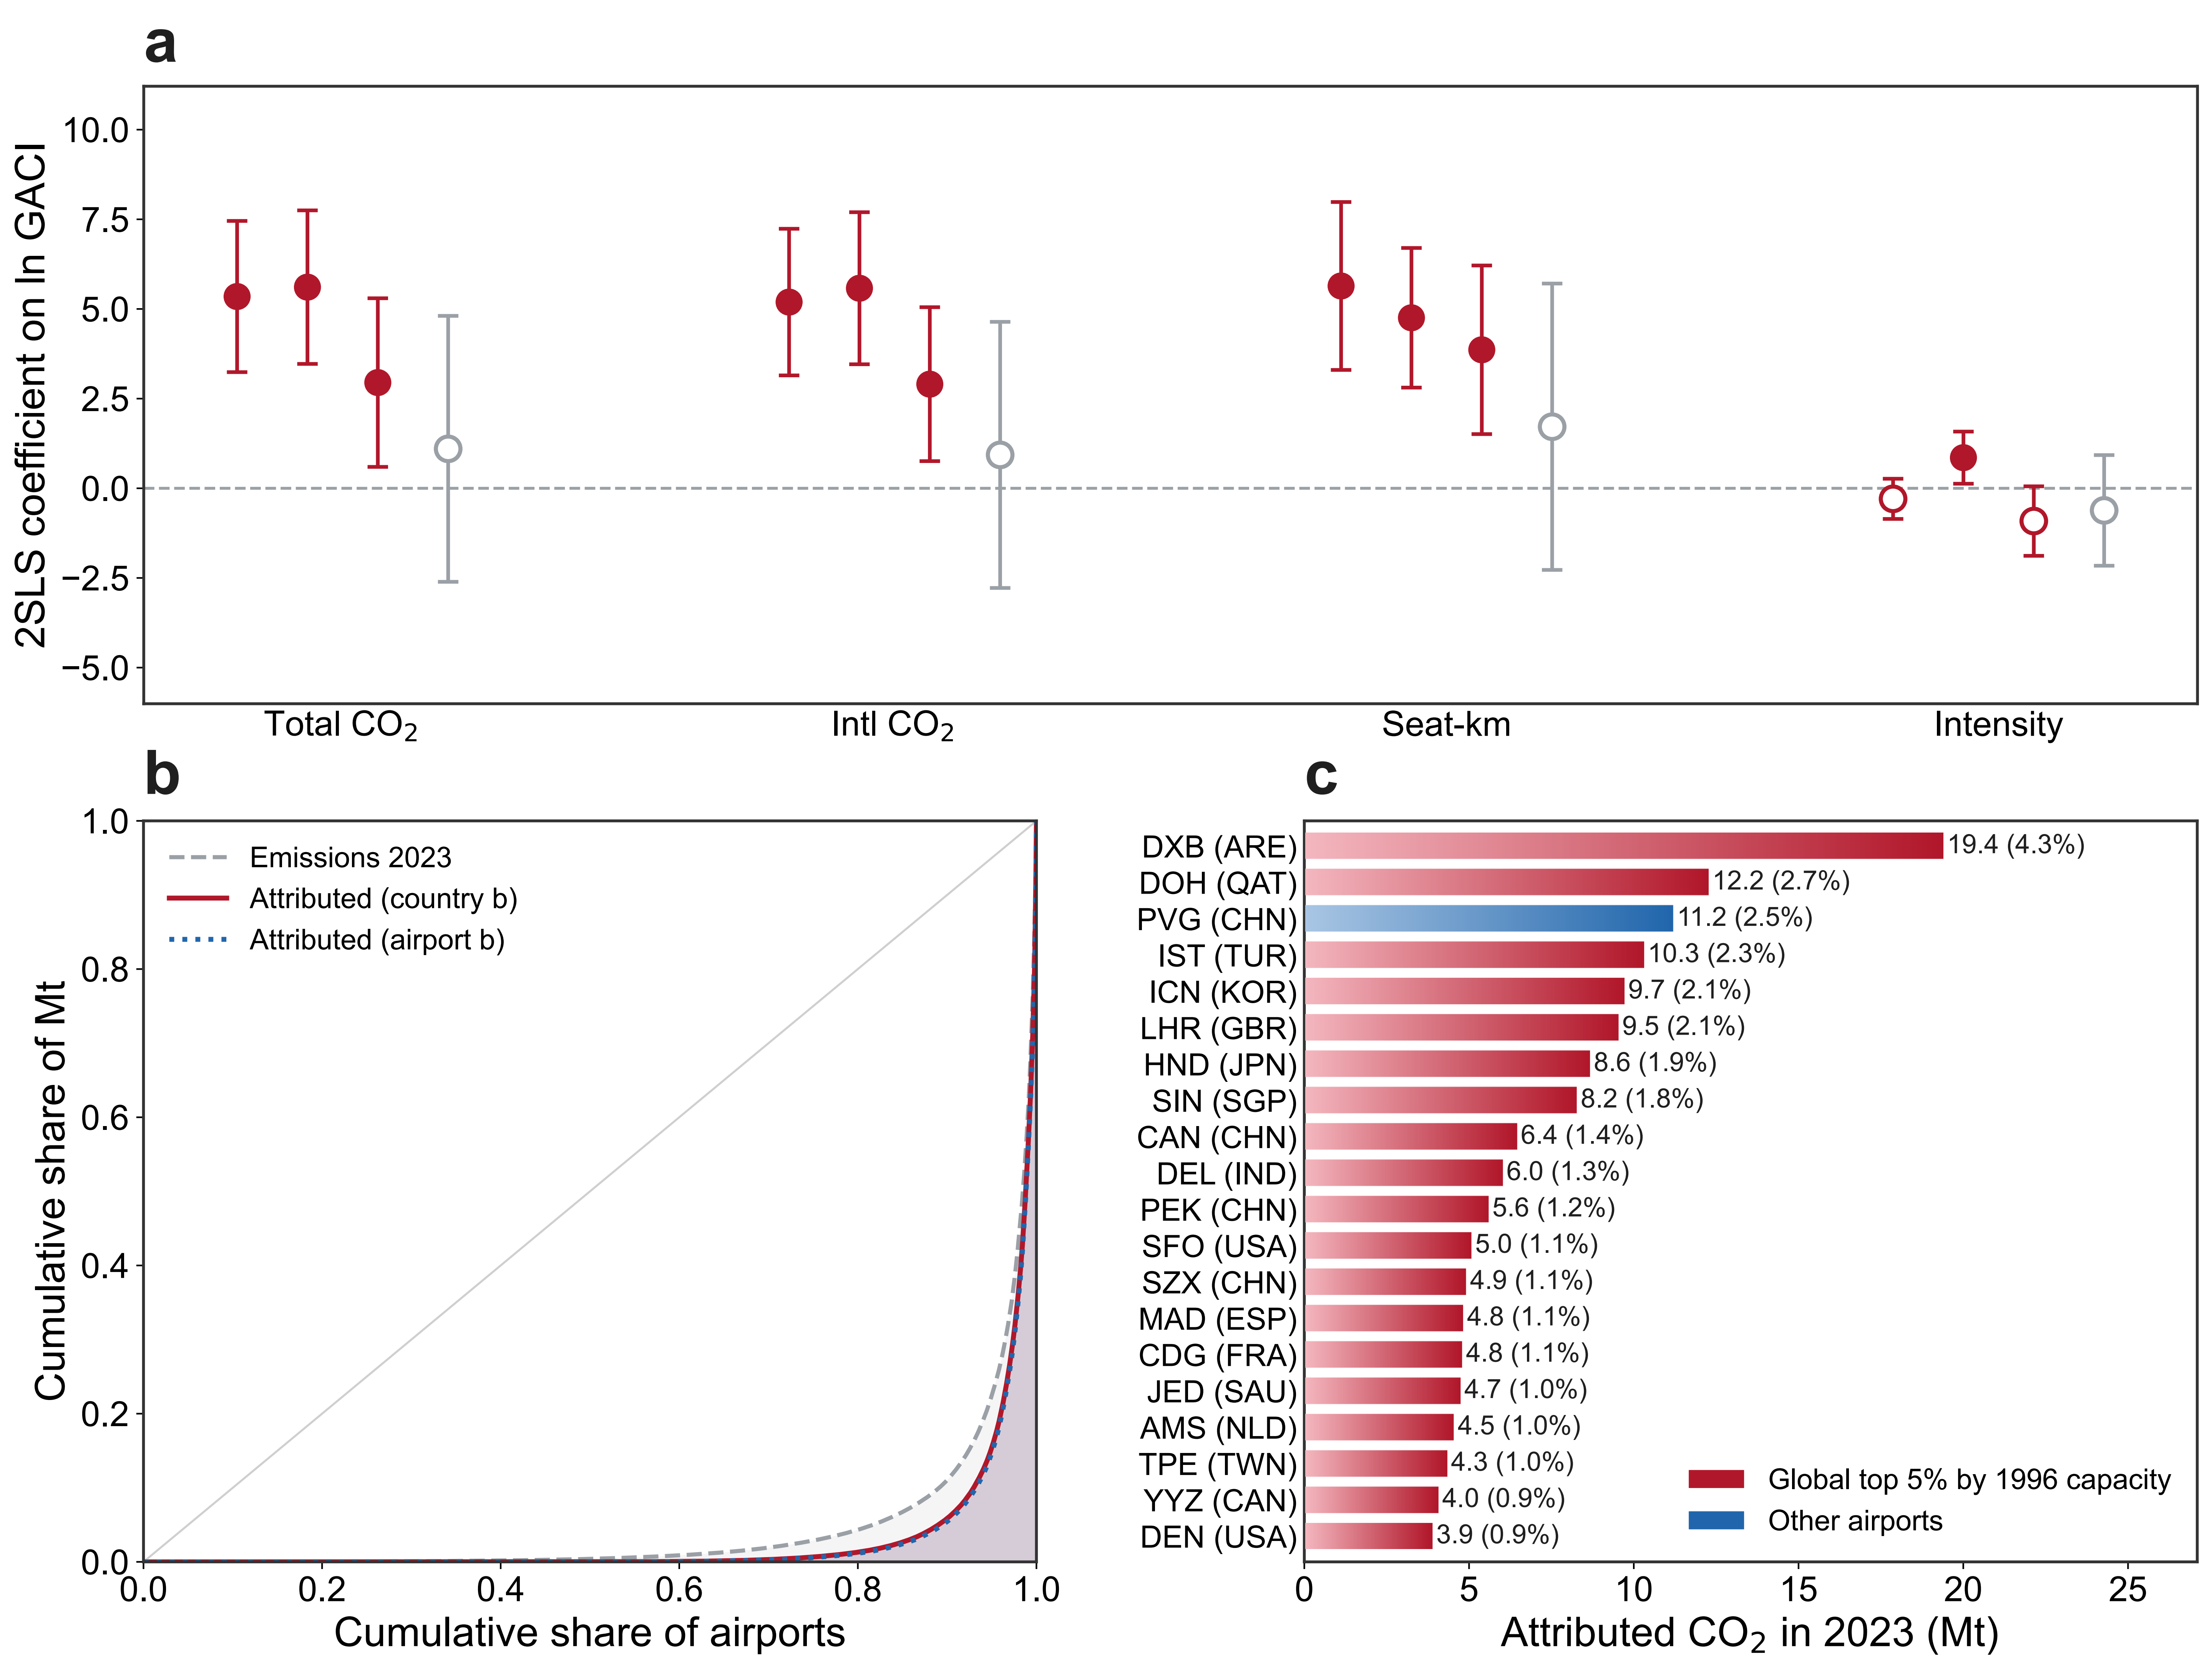
\includegraphics[width=0.95\textwidth]{ED_Fig1.png}
\caption{\textbf{Temporal split of the connectivity elasticity and concentration of connectivity-attributed emissions across airports.} \textbf{a}, Within each outcome, markers show the full sample, the network-expansion era (1996--2007), the mature-network era (2010--2023 excluding the COVID-19 years 2020--2021) and the unrestricted 2010--2023 sample from left to right. Filled markers denote $p<0.05$; grey denotes the unrestricted later sample, whose first stage (KP $F$ = 3.2) is contaminated by the COVID collapse. Bars are 95\% confidence intervals with standard errors clustered by country. \textbf{b}, Lorenz curves of 2023 emissions and of emissions attributed to 1996--2023 connectivity growth over 3{,}833 airports with positive emissions. \textbf{c}, The twenty largest attributed contributions in 2023 (Mt and share of the world attributed total); red marks airports in the global top five percent by 1996 capacity and blue the other airports.}
% Longfei: panel b currently also draws the curve based on the airport-level elasticity; that regression was removed from the paper (Junya, 2026-09-25). Please redraw with the country-elasticity curve only.
\label{fig:ed_temporal_airport}
\end{figure}

\begin{figure}[H]
\centering
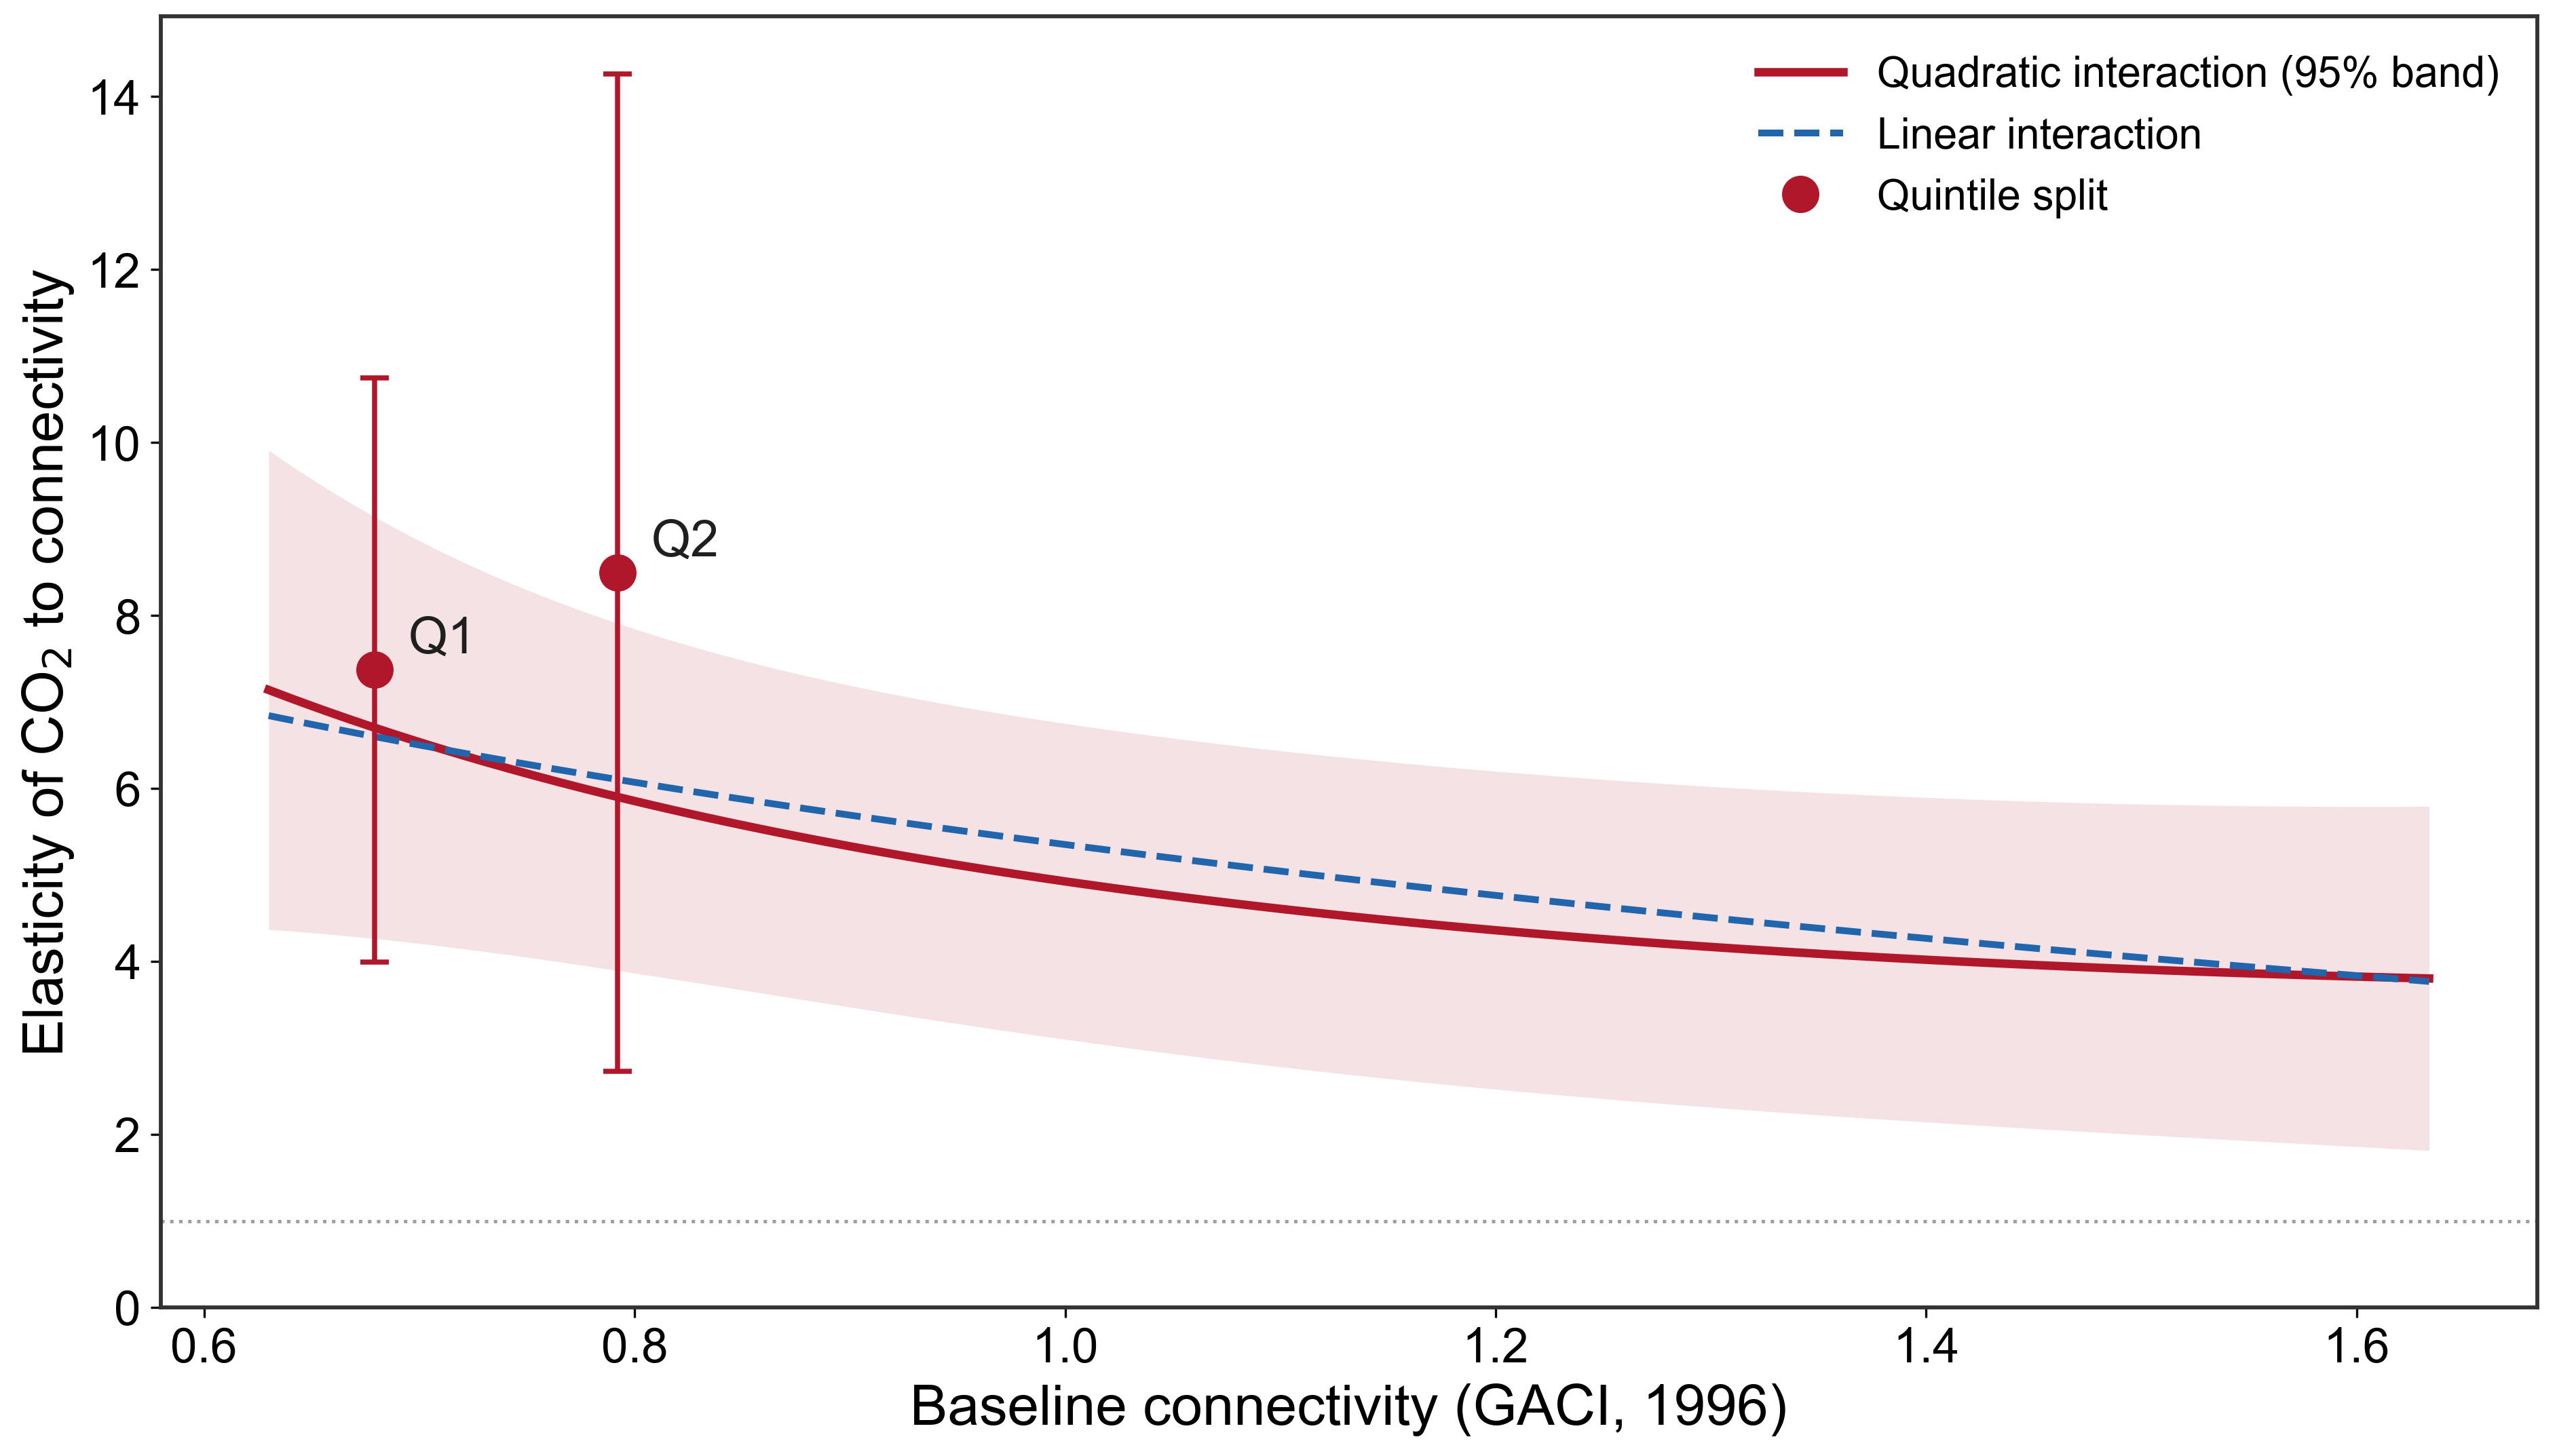
\includegraphics[width=0.85\textwidth]{ED_Fig2.png}
\caption{\textbf{The elasticity along the baseline-connectivity distribution.} Quintile split-sample 2SLS estimates for the two lowest quintiles (points, 95\% confidence intervals; the upper three quintiles have weak first stages, KP $F$ = 4.8, 0.0 and 2.1, and are reported in Extended Data Table~\ref{tab:gradient}) and the fitted elasticity from pooled specifications that interact log GACI with centred log baseline GACI (linear, dashed; quadratic with 95\% band). The dotted line marks an elasticity of one.}
\label{fig:gradient}
\end{figure}

\begin{figure}[H]
\centering
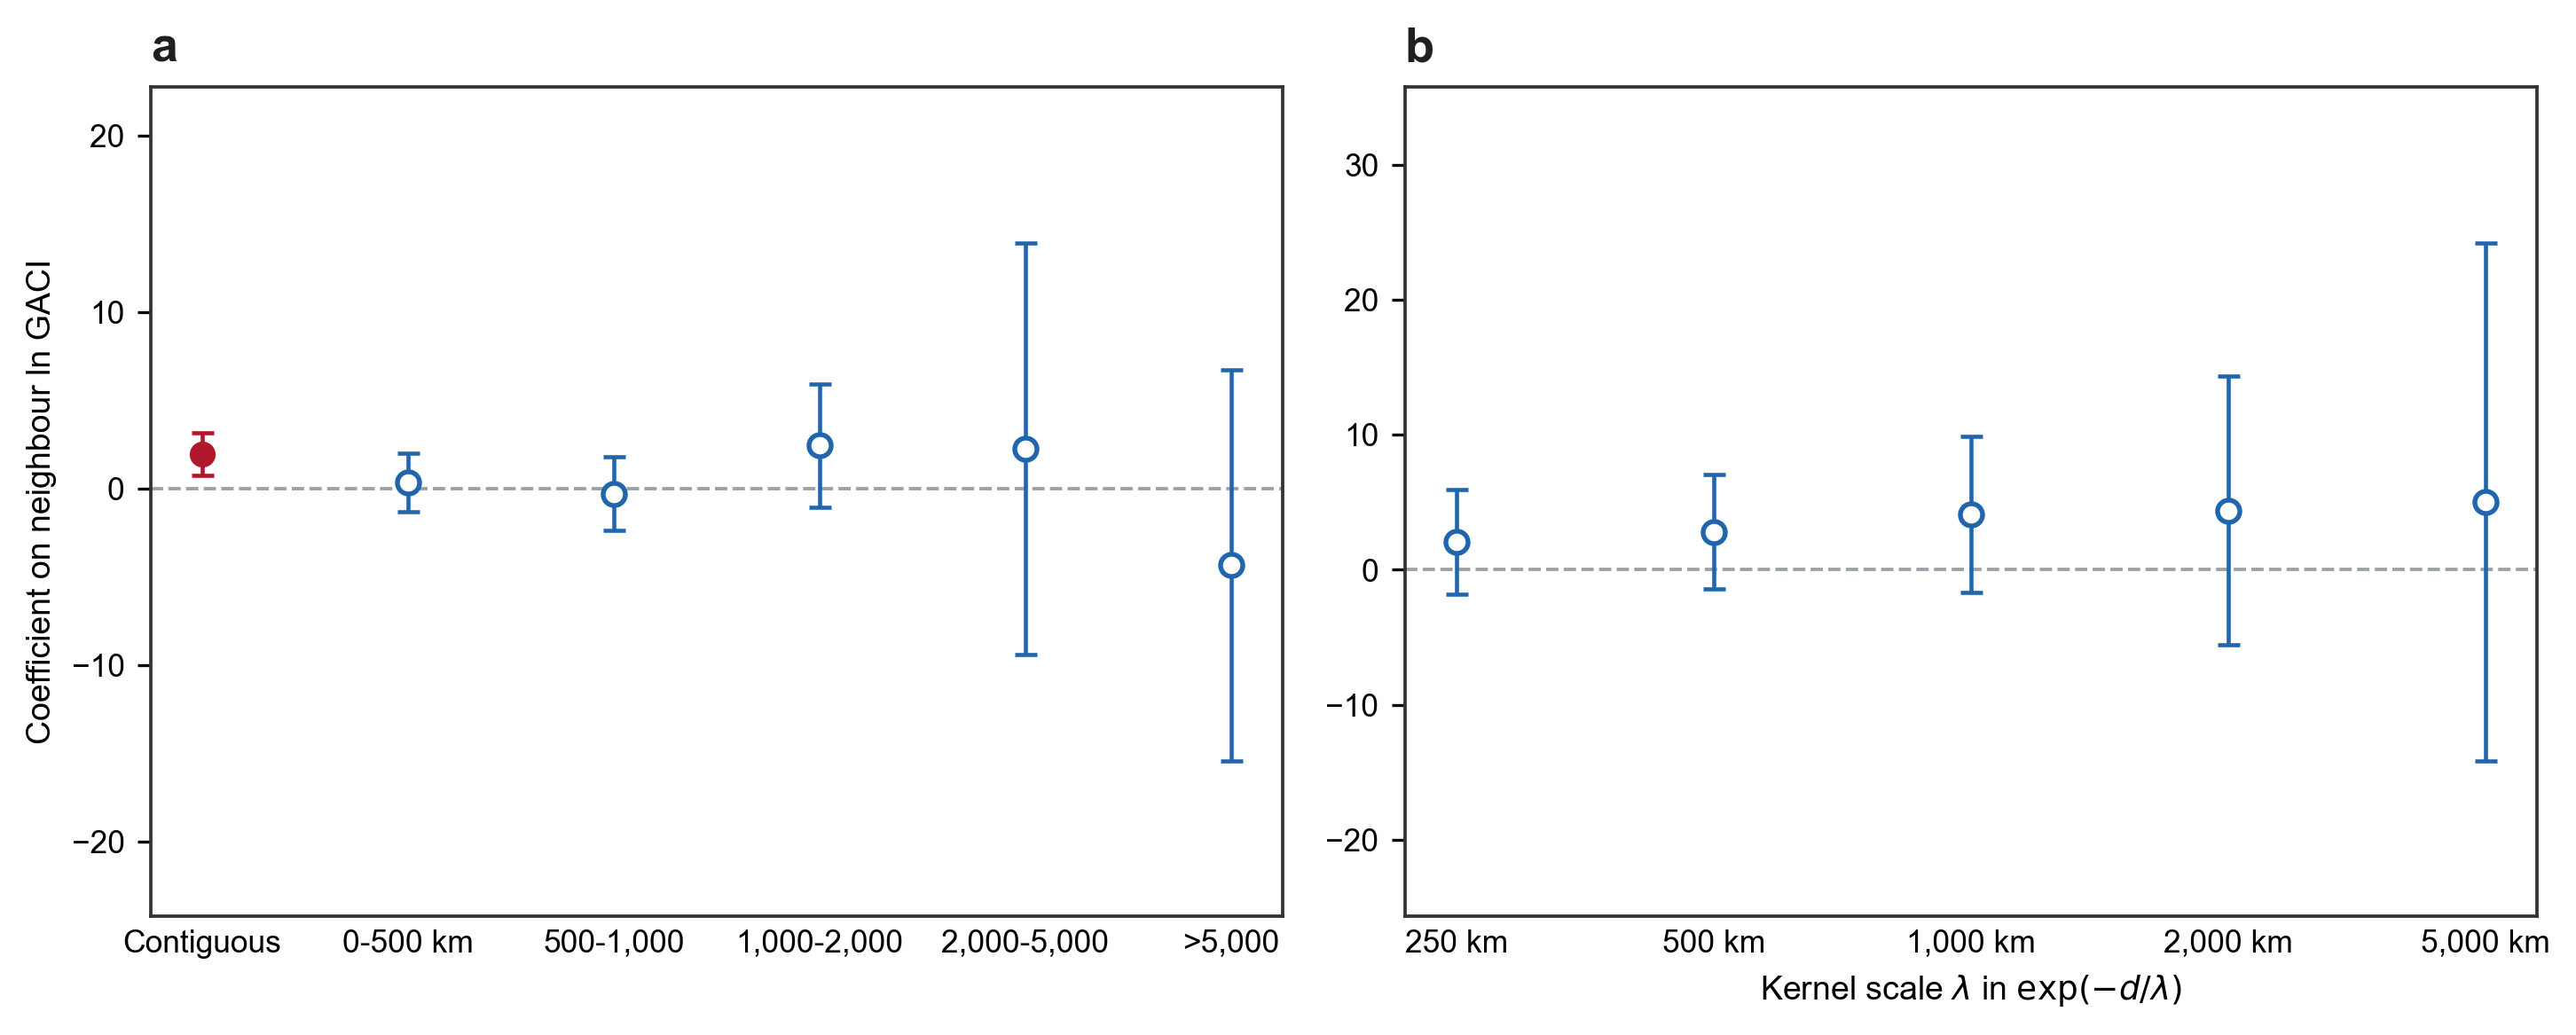
\includegraphics[width=0.95\textwidth]{ED_Fig3.png}
\caption{\textbf{Spatial profile of the spillover.} \textbf{a}, Coefficient on neighbour connectivity when one distance band at a time defines the neighbours (contiguous countries, then bands of aviation-centroid distance). \textbf{b}, The same with an exponential kernel of widening scale. Neighbour connectivity is instrumented by the identically weighted shifter and the own shifter is controlled. Filled markers denote $p<0.05$; bars are 95\% confidence intervals. The absence of a smooth decline and the negative but imprecise coefficient beyond 5{,}000 km indicate that wide exposures track global trends rather than a spatial spillover.}
\label{fig:spilldecay}
\end{figure}

\begin{figure}[H]
\centering
\includegraphics[width=0.95\textwidth]{ED_Fig4.png}
\caption{\textbf{Placebo tests for the spillover and for the instrument.} \textbf{a}--\textbf{c}, Permutation placebo for the spillover: distributions of the $t$-statistic on the neighbour term over 500 random relabellings of countries in the weight matrix for the inverse-distance reduced form (\textbf{a}) and the contiguity (\textbf{b}) and five-nearest (\textbf{c}) joint 2SLS specifications. The red line is the actual statistic, the shaded tails mark permuted statistics at least as large in absolute value, and $p$ is the permutation $p$-value. \textbf{d}, Reduced forms of the Feyrer instrument on aviation CO$_2$ (red) and on non-aviation emission series (blue), with 95\% confidence intervals; filled markers denote $p<0.05$. Specification as in Table~\ref{tab:main}. Coal and cement CO$_2$ are the two non-aviation series that respond (Methods).}
\label{fig:placebos}
\end{figure}

\clearpage
\section*{Supplementary Note 1: What the elasticity represents}
This note sets out why the headline elasticity of Table~\ref{tab:main}
describes the take-off stage of network development, using level
specifications, finer splits of the baseline distribution and the two
estimation eras (Extended Data Tables~\ref{tab:funcform} and
\ref{tab:gradient}; Extended Data Fig.~\ref{fig:gradient}).

The headline number describes the take-off stage of network development,
for three reasons. First, the gradient is not an artefact of the
logarithmic scale. Re-estimated with connectivity in levels (Extended
Data Table~\ref{tab:funcform}), the semi-log slope within
baseline-connectivity terciles is 9.1, 4.6 and 1.1 from bottom to top, so the same
absolute addition to the network raises emissions far more where the
network is thin. Second, the gradient is a step rather than a smooth
slope, and it is not confined to the very bottom of the distribution
(Extended Data Fig.~\ref{fig:gradient} and Extended Data
Table~\ref{tab:gradient}). Quintile splits give elasticities of 7.4 and
8.5 in the two lowest quintiles, 3.3 in the third and 4.0 in the fifth,
with the fourth unidentified. Third, the response is concentrated in the
expansion era: the elasticity falls from 5.6 to 2.9 between the
network-expansion and mature-network eras. The headline elasticity therefore describes
the emissions response during the take-off stage of national network
development, which the sample observes for most countries between 1996
and the late 2000s, rather than a universal constant.

\clearpage
\section*{Supplementary Note 2: Flight-level emissions inventory, country allocation and validation}
This note gives the full calculation behind the emissions inventory summarized in Methods.

\subsection*{Flight-level calculation}

We estimate flight-level CO$_2$ emissions from global scheduled flight records provided by the Official Airline Guide (OAG), covering January 1996 to June 2024, following the aviation emissions methodology of the European Monitoring and Evaluation Programme/European Environment Agency (EMEP/EEA) Air Pollutant Emission Inventory Guidebook \citep{eea2023} and using engine-specific operating parameters from the International Civil Aviation Organization (ICAO) Aircraft Engine Emissions Databank. For each physically operated flight leg $f$, total CO$_2$ emissions are separated into landing-and-take-off (LTO) and climb--cruise--descent (CCD) components:

\begin{equation}
E_{f,\mathrm{Total}}
=
E_{f,\mathrm{LTO}}
+
E_{f,\mathrm{CCD}} .
\label{eq:nature_1}
\end{equation}

The LTO component covers aircraft operations below 3,000 feet, while the CCD component covers climb, cruise and descent above 3,000 feet. In the EEA implementation used here, LTO emissions are calculated for five components: taxi-out, take-off, climb-out, approach and landing, and taxi-in. Multi-stop scheduled services are decomposed into their constituent operated legs before emissions are calculated, so that each physical leg contributes its own LTO and CCD emissions rather than being treated as a single end-to-end flight.

OAG equipment codes are matched to aircraft types and representative aircraft--engine configurations in the EEA aviation emissions database. Where an exact aircraft type is unavailable, we assign a representative type from the same aircraft family or series, or the closest operational substitute on the basis of aircraft size and operating characteristics. The resulting aircraft--engine mapping links each scheduled flight leg to the aircraft-specific parameters required for the LTO and CCD calculations.

For LTO emissions, we retain the five operating components separately. Let $j(f)$ denote the aircraft--engine configuration assigned to flight $f$, and let $k$ index the five LTO components. CO$_2$ emissions for component $k$ are calculated as

\begin{equation}
\begin{aligned}
E_{f,k}^{\mathrm{LTO}}
&=
T_k
\,FF_{j(f),k}
\,NE_{j(f)}
\,EF_{\mathrm{CO_2}},
&
E_{f,\mathrm{LTO}}
&=
\sum_{k\in\mathcal K_{\mathrm{LTO}}}
E_{f,k}^{\mathrm{LTO}}.
\end{aligned}
\label{eq:nature_2}
\end{equation}

where $T_k$ is the standard time in mode, $FF_{j(f),k}$ is the fuel-flow rate per engine for the corresponding operating mode, $NE_{j(f)}$ is the number of engines, and $EF_{\mathrm{CO_2}}$ is the fuel-specific CO$_2$ emission factor. We use standard time-in-mode values of 19 minutes for taxi-out, 0.7 minutes for take-off, 2.2 minutes for climb-out, 4 minutes for approach and landing, and 7 minutes for taxi-in. Engine-specific fuel-flow rates are obtained from the International Civil Aviation Organization (ICAO) Aircraft Engine Emissions Databank. CO$_2$ emission factors are 3.15 kilograms of CO$_2$ per kilogram of Jet A and 3.10 kilograms of CO$_2$ per kilogram of aviation gasoline. Retaining the individual LTO components also allows departure- and arrival-side emissions to be distinguished in the country-level allocation described below.

CCD emissions are estimated from aircraft-specific reference values provided by the EEA at discrete flight distances. For each flight leg, great-circle distance between the origin and destination airports is converted to the corresponding EEA flight distance following \citet{avogadro2024}. When this distance $d_f$ falls between two adjacent EEA reference distances $d_1$ and $d_2$, CCD emissions are obtained by linear interpolation:

\begin{equation}
\begin{split}
E_{f,\mathrm{CCD}}(d_f)
={}&
E_{j(f),\mathrm{CCD}}(d_1)\\
&+
\left[
E_{j(f),\mathrm{CCD}}(d_2)
-
E_{j(f),\mathrm{CCD}}(d_1)
\right]
\frac{d_f-d_1}{d_2-d_1}.
\end{split}
\label{eq:nature_3}
\end{equation}

This procedure preserves the aircraft-specific EEA fuel-burn relationships while allowing emissions to vary continuously with flight distance. The resulting inventory therefore provides standardized LTO- and CCD-specific CO$_2$ estimates for each scheduled flight leg, rather than attempting to reproduce realized trajectories or flight-specific meteorological and operational conditions.

\subsection*{Allocation of emissions to countries}

Constructing country-year emissions from the flight-level inventory requires an explicit rule for attributing emissions to national units. This is relatively straightforward for LTO emissions, because the underlying operations can be associated with the departure or arrival airport. The attribution of CCD emissions is less direct, particularly for international flights, because the en-route component does not have a unique country assignment. Country-level aviation emissions therefore depend in part on the accounting convention used to allocate this component. To separate locally anchored airport emissions from this accounting choice, and to assess the sensitivity of our empirical results to alternative treatments of international en-route emissions, we construct three country-level measures.

Because the five LTO components are retained separately in the flight-level inventory, we distinguish the emissions associated with the departure and arrival sides of each flight. For flight leg $f$, define

\[
D_f
=
E_{f,\mathrm{taxi\mbox{-}out}}
+
E_{f,\mathrm{take\mbox{-}off}}
+
E_{f,\mathrm{climb\mbox{-}out}},
\]

\[
A_f
=
E_{f,\mathrm{approach/landing}}
+
E_{f,\mathrm{taxi\mbox{-}in}},
\qquad
C_f
=
E_{f,\mathrm{CCD}}.
\]

Total emissions from the flight leg can therefore be written as

\begin{equation}
E_{f,\mathrm{Total}}
=
D_f+A_f+C_f .
\label{eq:nature_4}
\end{equation}

For a flight from airport $A$ to airport $B$, $D_f$ is assigned to the country containing the departure airport and $A_f$ to the country containing the arrival airport. This links LTO emissions to the location of the corresponding airport operation. Flights are classified as domestic or international according to whether their origin and destination airports are located in the same country. The three national measures differ only in their treatment of $C_f$.

The first is an LTO-only measure, which attributes to each country only the emissions associated with airport operations occurring at its airports. Let $O_{ct}$ and $I_{ct}$ denote the sets of flight legs departing from and arriving in country $c$ in year $t$, respectively. We define

\begin{equation}
E^{\mathrm{LTO}}_{ct}
=
\sum_{f\in O_{ct}}D_f
+
\sum_{f\in I_{ct}}A_f .
\label{eq:nature_5}
\end{equation}

Because this measure excludes CCD emissions by construction, it is not intended to represent a complete national aviation-emissions inventory. Rather, it provides a geographically anchored measure of local aviation emissions that is independent of any convention for allocating the en-route component of international flights.

Our headline measure additionally assigns the full CCD component of each flight to its country of departure:

\begin{equation}
E^{\mathrm{dep}}_{ct}
=
E^{\mathrm{LTO}}_{ct}
+
\sum_{f\in O_{ct}} C_f .
\label{eq:nature_6}
\end{equation}

We refer to this as the departure-based, or bunker, measure. At the flight level, this allocation mirrors the origin-side logic of international bunker accounting: en-route emissions are associated with the departing side of the flight, while LTO emissions remain assigned to the airports at which the corresponding operations occur. The measure therefore provides a complete allocation of flight emissions across countries and serves as the principal emissions outcome in the empirical analysis.

As a symmetric alternative, we construct a 50/50 measure that assigns one half of each flight's CCD emissions to the origin country and the other half to the destination country:

\begin{equation}
E^{50/50}_{ct}
=
E^{\mathrm{LTO}}_{ct}
+
\frac{1}{2}\sum_{f\in O_{ct}} C_f
+
\frac{1}{2}\sum_{f\in I_{ct}} C_f .
\label{eq:nature_7}
\end{equation}

This allocation does not privilege either endpoint in assigning international en-route emissions and therefore provides a transparent robustness check on the origin-based convention.

For domestic flights, the departure-based and 50/50 measures are identical because both endpoints belong to the same country. Differences between the two full-emissions measures therefore arise entirely from the allocation of CCD emissions on international flights. Importantly, both allocation rules preserve the same global emissions total:

\begin{equation}
\sum_c E^{\mathrm{dep}}_{ct}
=
\sum_c E^{50/50}_{ct}
=
\sum_{f\in F_t}
\left(D_f+A_f+C_f\right),
\label{eq:nature_8}
\end{equation}

where $F_t$ denotes all flight legs in year $t$. Thus, differences across the national measures reflect only how a fixed quantity of flight-level emissions is distributed across countries, rather than differences in the underlying emissions inventory.

\subsection*{Validation against external benchmarks}

The flight-level inventory is intended to provide globally consistent estimates over nearly three decades rather than to reproduce the realized conditions of every individual flight. Meteorological conditions, routing and air-traffic-control adjustments, airport-specific operations, and other flight-level variation are therefore not observed, and a small number of aircraft types are represented by closely matched aircraft--engine configurations when no exact EEA counterpart is available. Standardized time-in-mode and aircraft-performance parameters likewise represent typical rather than realized operations. We therefore assess whether these approximations materially affect the dimensions of the inventory used in our analysis: the scale of emissions, their geographic distribution, and their LTO--CCD composition.

The scale and evolution of global aviation emissions are closely reproduced against two references constructed from fundamentally different sources. The International Air Transport Association (IATA) provides industry-level global CO$_2$ estimates based on airline operational and industry statistics, whereas the Organisation for Economic Co-operation and Development (OECD) constructs a bottom-up inventory from individual flight activity and engineering-based emissions calculations \citep{iata2018,iata2019,iata2024,clarke2022}. The convergence of these distinct approaches is informative because it does not arise from alternative implementations of the same underlying model. Over 2004--2023, our estimates have a weighted absolute percentage error (WAPE) of 3.04\% relative to IATA and an aggregate bias of $-1.98\%$; against the OECD inventory over 2013--2023, the corresponding values are 3.58\% and $+3.40\%$ (Extended Data Table~\ref{tab:validation_benchmarks}).

IATA and OECD provide global coverage but remain estimated emissions series. We therefore complement them with carrier-reported fuel consumption from the United States (U.S.) Bureau of Transportation Statistics (BTS), which is geographically narrower but more directly measures the physical quantity underlying CO$_2$ emissions. Over 1996--2023, our estimated U.S.-carrier fuel consumption has a WAPE of 3.84\% relative to BTS and an aggregate bias of $+0.76\%$. Together, the three sources test the inventory from complementary perspectives: global industry estimates, an independent flight-level inventory, and reported fuel use.

We next examine the cross-country distribution of emissions, which is directly relevant to the country-year empirical design. After applying a consistent departure-country allocation rule, the mean annual log-scale Pearson correlation with the OECD territory-based series is 0.999 over 2013--2018, with a mean total variation distance (TVD) of 1.05\%. From 2019, when the OECD activity data shift from scheduled-flight records to realized flights observed through Automatic Dependent Surveillance--Broadcast (ADS-B), agreement remains strong but discrepancies increase: over 2019--2023, the mean correlation is 0.955 and mean TVD is 6.04\%. Matched countries account for more than 99\% of emissions in our inventory in every year. The post-2019 divergence is therefore consistent with differences between scheduled and realized flight activity rather than a broad disagreement in the geographic distribution of emissions.

Finally, the estimated flight-phase composition is also consistent with independent evidence. LTO operations account for 12.41\% of total CO$_2$ emissions over 1996--2023. \citet{quadros2022} report global LTO fuel-burn shares of 10.8--13.5\% under ICAO reference LTO-cycle assumptions. Because CO$_2$ emissions from conventional aviation fuel are proportional to fuel burn, these values provide a directly comparable reference, and our estimate falls within the reported range.

\clearpage
\section*{Supplementary Note 3: Construction of the Global Air Connectivity Index}
This note defines the network measures and the aggregation behind GACI, following \citet{cheung2020}; Methods gives the summary.

Let $V_t$ denote the set of airports with active scheduled service in year $t$. Airports are represented as nodes and scheduled connections as undirected links, with $a_{ijt}=1$ if airports $i$ and $j$ are directly connected and zero otherwise. Let $q_{ijt}$ denote annual scheduled seat capacity on the link, aggregated over both directions. Airport strength and degree are

\begin{equation}
s_{it}
=
\sum_{j\in V_t} q_{ijt},
\qquad
d_{it}
=
\sum_{j\in V_t} a_{ijt}.
\label{eq:nature_9}
\end{equation}

For each active link $\{i,j\}$, connection intensity is defined as

\begin{equation}
w_{ijt}
=
\sqrt{
\frac{s_{it}s_{jt}}
{d_{it}d_{jt}}
},
\qquad
a_{ijt}=1,
\label{eq:nature_10}
\end{equation}

and $w_{ijt}=0$ otherwise. This measure is high when both endpoint airports carry substantial scheduled capacity per connection and provides the common measure of connection strength used in the weighted components of GACI.

GACI combines five complementary indicators of airport network position.

Degree measures the number of airports directly connected to airport $i$:

\begin{equation}
d_{it}
=
\sum_{j\in V_t} a_{ijt}.
\label{eq:nature_11}
\end{equation}

It captures the direct reach of an airport within the global network.

Flow betweenness captures the extent to which airport $i$ lies on potential transfer flows between other origin--destination pairs:

\begin{equation}
F_b(i,t)
=
\frac{1}{N_{B,t}}
\sum_{\substack{j,g\in V_t\\
j\neq g,\; j\neq i,\; g\neq i}}
\tau_{jgt}(i),
\qquad
N_{B,t}
=
\frac{N_t(N_t-1)}{2},
\label{eq:nature_12}
\end{equation}

where $N_t=|V_t|$ and $\tau_{jgt}(i)$ denotes modelled flow through airport $i$ between airports $j$ and $g$ under an electrical-circuit representation of the weighted network, with link conductance proportional to $w_{ijt}$. The measure therefore captures an airport's importance as an intermediary in the network rather than only its direct connections.

Closeness centrality measures the topological accessibility of airport $i$:

\begin{equation}
C_c(i,t)
=
\frac{N_t-1}
{\displaystyle
\sum_{\substack{j\in V_t\\j\neq i}}
\mathrm{Dist}_t(i,j)
},
\label{eq:nature_13}
\end{equation}

where $\mathrm{Dist}_t(i,j)$ is the shortest-path length between airports $i$ and $j$, measured in flight legs. Closeness therefore reflects how few connections are required to reach the rest of the network rather than geographic distance, flight distance or travel time.

Eigenvector centrality assigns greater weight to connections with airports that are themselves highly connected:

\begin{equation}
C_E(i,t)
=
\frac{1}{\lambda_t}
\sum_{j\in V_t}
w_{ijt} C_E(j,t),
\label{eq:nature_14}
\end{equation}

where $\lambda_t$ is the largest eigenvalue of the weighted adjacency matrix $W_t=[w_{ijt}]$. Connections to more central airports therefore contribute more strongly to an airport's network importance.

Finally, regional importance captures the strength of an airport's connections within its own OAG world region. Let $R(i)$ denote the region containing airport $i$, and define

\begin{equation}
V^R_{it}
=
\left\{
j\in V_t:
a_{ijt}=1,\;
R(j)=R(i)
\right\}.
\label{eq:nature_15}
\end{equation}

Regional importance is

\begin{equation}
C_R(i,t)
=
\frac{1}{|V^R_{it}|}
\sum_{j\in V^R_{it}}
w_{ijt}.
\label{eq:nature_16}
\end{equation}

This component measures the strength of an airport's position within its regional aviation network. Taken together, degree, closeness and eigenvector centrality primarily characterize network topology, whereas flow betweenness and regional importance additionally incorporate the intensity of airport connections. The five measures therefore capture distinct but complementary dimensions of connectivity.

Because the five indicators differ in scale, they are standardized following \citet{cheung2020} and combined using principal component analysis (PCA). Let $\tilde d_{it}$, $\tilde f_{it}$, $\tilde c_{it}$, $\tilde e_{it}$ and $\tilde r_{it}$ denote the standardized degree, flow-betweenness, closeness, eigenvector-centrality and regional-importance measures. Airport-level GACI is defined by the first principal component:

\begin{equation}
\mathrm{GACI}_{it}
=
\begin{bmatrix}
\tilde d_{it} &
\tilde f_{it} &
\tilde c_{it} &
\tilde e_{it} &
\tilde r_{it}
\end{bmatrix}
\boldsymbol{\alpha}_t ,
\label{eq:nature_17}
\end{equation}

where $\boldsymbol{\alpha}_t$ is the first-principal-component loading vector estimated for the year-$t$ network. Across 1996--2023, the loadings are uniformly positive and highly stable, and the first component explains 63--77\% of annual variation in the five standardized indicators. A pooled PCA estimated over all airport-year observations yields an index correlated at 0.98 with the year-specific construction, supporting the intertemporal comparability of the index.

We additionally consider three alternative aggregations. The maximum

\begin{equation}
\mathrm{GACI}^{\max}_{ct}
=
\max_{i\in A_{ct}}
\mathrm{GACI}_{it}
\label{eq:nature_19}
\end{equation}

captures the connectivity of the country's leading gateway. The sum

\begin{equation}
\mathrm{GACI}^{\mathrm{sum}}_{ct}
=
\sum_{i\in A_{ct}}
\mathrm{GACI}_{it}
\label{eq:nature_20}
\end{equation}

captures aggregate airport-system connectivity, whereas the unweighted mean

\begin{equation}
\mathrm{GACI}^{\mathrm{mean}}_{ct}
=
\frac{1}{|A_{ct}|}
\sum_{i\in A_{ct}}
\mathrm{GACI}_{it}
\label{eq:nature_21}
\end{equation}

assigns equal weight to all active airports. The capacity-weighted mean is our headline measure; the alternative aggregations assess the robustness of the results to different representations of national network structure.

\section*{Supplementary Tables}
\setcounter{table}{0}
\renewcommand{\tablename}{Supplementary Table}

\begin{table}[H]
\centering
\adjustbox{max width=\textwidth, max totalheight=0.9\textheight}{%
\begin{threeparttable}
\caption{Summary statistics, estimation sample}
\label{tab:sumstat}
\scriptsize
\begin{tabular}{lrrrrr}
\toprule
Variable & $N$ & Mean & s.d. & Min & Max \\
\midrule
\multicolumn{6}{l}{\textit{Panel A. Aviation outcomes}} \\
  Aviation CO$_2$, bunker convention (Mt) & 4,634 & 3.82 & 15.49 & $<$0.01 & 206.14 \\
  International aviation CO$_2$ (Mt) & 4,634 & 2.29 & 6.21 & $<$0.01 & 77.75 \\
  Domestic aviation CO$_2$ (Mt) & 3,575 & 1.98 & 11.55 & $<$0.01 & 148.11 \\
  Aviation CO$_2$, territorial LTO rule (Mt) & 4,634 & 0.47 & 1.95 & $<$0.01 & 28.26 \\
  Aviation CO$_2$, 50/50 rule (Mt) & 4,634 & 3.82 & 15.47 & $<$0.01 & 205.87 \\
  Departing seat-km (billion) & 4,634 & 38.24 & 152.02 & $<$0.01 & 2,267.76 \\
  Departing flights (thousand) & 4,634 & 182.4 & 847.2 & $<$0.1 & 12,213.7 \\
  Seats per flight & 4,634 & 121.2 & 43.1 & 12.0 & 281.1 \\
  Km per seat (average stage length) & 4,634 & 1,591 & 705 & 248 & 5,178 \\
  CO$_2$ per seat-km (g) & 4,634 & 112.0 & 63.9 & 58.7 & 1,176.1 \\
  LTO share of CO$_2$ & 4,634 & 0.150 & 0.052 & 0.047 & 0.443 \\
  International share of seat-km & 4,634 & 0.882 & 0.168 & 0.024 & 1.000 \\
\multicolumn{6}{l}{\textit{Panel B. Connectivity (log GACI)}} \\
  ln GACI, capacity-weighted mean (headline) & 4,634 & 0.025 & 0.323 & $-$0.628 & 1.103 \\
  ln GACI, sum & 4,634 & 1.534 & 1.357 & $-$0.606 & 6.234 \\
  ln GACI, maximum & 4,634 & 0.138 & 0.402 & $-$0.628 & 1.288 \\
  ln GACI, unweighted mean & 4,634 & $-$0.280 & 0.227 & $-$0.819 & 1.081 \\
\multicolumn{6}{l}{\textit{Panel C. Instrument and baseline controls}} \\
  Instrument $Z_{ct}=a_t\times\ln \mathrm{airMA}_{c,1996}$ & 4,634 & 4.863 & 4.381 & 0.000 & 14.667 \\
  World aviation index $a_t$ (0--1) & 4,634 & 0.352 & 0.317 & 0.000 & 1.000 \\
  ln air market access, 1996 & 4,634 & 13.822 & 0.367 & 12.996 & 14.667 \\
  ln sea market access & 4,634 & 13.766 & 0.365 & 12.832 & 14.806 \\
  Population (million) & 4,634 & 39.39 & 144.65 & 0.01 & 1,438.07 \\
\multicolumn{6}{l}{\textit{Panel D. Development controls}} \\
  GDP (billion current US\$) & 4,634 & 375.6 & 1,575.1 & 0.1 & 27,292.2 \\
  Trade (\% of GDP) & 4,602 & 86.8 & 52.9 & 2.5 & 442.6 \\
  Urban population (\% of total) & 4,634 & 59.4 & 22.8 & 10.3 & 100.0 \\
  FDI net inflows (\% of GDP) & 4,449 & 5.2 & 22.2 & $-$391.6 & 452.2 \\
  International tourist arrivals (million) & 3,584 & 10.02 & 24.86 & $<$0.01 & 217.88 \\
\multicolumn{6}{l}{\textit{Panel E. Non-aviation placebo outcomes (log Mt CO$_2$)}} \\
  Territorial fossil CO$_2$ excl.\ domestic aviation (GCP/OWID) & 4,576 & 2.683 & 2.423 & $-$3.851 & 9.377 \\
  Oil CO$_2$ excl.\ domestic aviation (OWID) & 4,576 & 2.046 & 2.123 & $-$3.851 & 7.828 \\
  Transport CO$_2$ excl.\ domestic aviation (EDGAR) & 4,461 & 1.450 & 2.147 & $-$6.989 & 7.426 \\
  Power industry CO$_2$ (EDGAR) & 4,409 & 1.246 & 2.866 & $-$10.516 & 8.775 \\
  Buildings CO$_2$ (EDGAR) & 4,460 & 0.343 & 2.557 & $-$8.699 & 6.586 \\
  Industrial combustion CO$_2$ (EDGAR) & 4,432 & 0.622 & 2.562 & $-$6.082 & 8.037 \\
  Coal CO$_2$ (OWID) & 3,034 & 1.255 & 3.122 & $-$6.908 & 9.054 \\
  Gas CO$_2$ (OWID) & 2,864 & 2.130 & 2.523 & $-$6.908 & 7.471 \\
  Cement CO$_2$ (OWID) & 3,476 & 0.237 & 1.880 & $-$6.908 & 6.745 \\
  Agriculture CO$_2$ (EDGAR) & 2,667 & $-$1.529 & 2.032 & $-$8.471 & 3.438 \\
\multicolumn{6}{l}{\textit{Panel F. Spatial exposures (row-normalized land contiguity)}} \\
  Neighbours' ln GACI, $W\ln\mathrm{GACI}$ & 3,725 & 0.091 & 0.249 & $-$0.396 & 0.858 \\
  Neighbours' instrument, $WZ$ & 3,725 & 4.817 & 4.375 & 0.000 & 14.373 \\
  Has a land neighbour (0/1) & 4,634 & 0.804 & 0.397 & 0.000 & 1.000 \\
\bottomrule
\end{tabular}
\begin{tablenotes}[flushleft]
\scriptsize
\item Notes: Estimation sample of Table~\ref{tab:main} (182 countries, 1996--2023, 4,634 country-years). Aviation variables are computed from the OAG flight-level inventory (Methods); km per seat is departing seat-kilometres divided by departing seats, and domestic CO$_2$ is reported for country-years with positive domestic emissions. GACI aggregations follow equations~\ref{eq:nature_18}--\ref{eq:nature_21}; air and sea market access follow equation~\ref{eq:seama}, and $a_t$ is world scheduled seat capacity (OAG), min--max scaled over 1996--2023. Development controls are from the World Bank World Development Indicators; Venezuela's trade share for 1996--2011, reported as zero, is treated as missing. Placebo outcomes are from the Global Carbon Project via Our World in Data and from EDGAR (2024 edition), with domestic aviation CO$_2$ from our inventory subtracted where stated. Neighbour exposures are reported for the 3,725 country-years with at least one land neighbour. Minima below display precision are shown as $<$0.01.
\end{tablenotes}
\end{threeparttable}}
\end{table}

\begin{table}[H]
\centering
\adjustbox{max width=\textwidth, max totalheight=0.9\textheight}{%
\begin{threeparttable}
\caption{Alternative technology series, distance decay and inference}
\label{tab:exclusion2}
\scriptsize
\begin{tabular}{lcccc}
\toprule
 & First-stage $\pi$ & 2SLS & KP $F$ & $N$ \\
\midrule
\multicolumn{5}{l}{\textit{Panel A. Technology series in the interaction (all $\times$ log 1996 air market access)}} \\
  World seat capacity (baseline) & 0.128$^{***}$ (0.030) & 5.35$^{***}$ (1.08) & 18.4 & 4,634 \\
  World flights & 0.128$^{***}$ (0.031) & 5.25$^{***}$ (1.17) & 17.2 & 4,634 \\
  World seat-km & 0.147$^{***}$ (0.033) & 5.38$^{***}$ (1.05) & 19.6 & 4,634 \\
  World sum of GACI & 0.137$^{***}$ (0.031) & 5.64$^{***}$ (1.02) & 19.5 & 4,634 \\
  World fuel-efficiency index (CO$_2$ per seat-km, inverted) & 0.160$^{***}$ (0.035) & 5.62$^{***}$ (0.98) & 21.3 & 4,634 \\
  Baseline geography recomputed ($\theta = 1$) & 0.127$^{***}$ (0.029) & 5.55$^{***}$ (1.10) & 19.3 & 4,634 \\
  Distance decay $\theta = 0.5$ & 0.274$^{***}$ (0.064) & 5.36$^{***}$ (1.09) & 18.2 & 4,634 \\
  Distance decay $\theta = 1.5$ & 0.073$^{***}$ (0.017) & 5.82$^{***}$ (1.18) & 18.0 & 4,634 \\
\midrule
\multicolumn{5}{l}{\textit{Panel B. Inference (2SLS on log CO$_2$)}} \\
 & 2SLS & s.e. & KP $F$ & $N$ \\
  Heteroskedasticity-robust & 5.35$^{***}$ & (0.40) & 153.6 & 4,634 \\
  Clustered by country (baseline) & 5.35$^{***}$ & (1.08) & 18.4 & 4,634 \\
  Two-way clustered (country, year) & 5.35$^{***}$ & (1.07) & 15.6 & 4,634 \\
\bottomrule
\end{tabular}
\begin{tablenotes}\scriptsize
\item Specification as in Table~\ref{tab:main}, column 1. Panel A replaces the world seat-capacity index $a_t$ by other world aviation series, each min--max scaled over 1996--2023: world departing flights, world departing seat-kilometres and the world sum of airport GACI from the OAG schedules, and a fuel-efficiency index equal to minus the log of world CO$_2$ per seat-kilometre in our inventory; the last three rows recompute 1996 air market access with the stated distance-decay exponent $\theta$ (baseline $\theta=1$; equation~\ref{eq:seama}). Panel B compares standard-error estimators for the baseline specification. $^{***}$ $p<0.01$, $^{**}$ $p<0.05$, $^{*}$ $p<0.1$.
\end{tablenotes}
\end{threeparttable}}
\end{table}

\begin{table}[H]
\centering
\adjustbox{max width=\textwidth, max totalheight=0.9\textheight}{%
\begin{threeparttable}
\caption{Aviation-accident instrument (Aviation Safety Network), pilot}
\label{tab:accident_iv}
\footnotesize
\begin{tabular}{lcccc}
\toprule
 & Bunker CO$_2$ & Intl.\ CO$_2$ & Intensity & KP $F$ \\
\midrule
  2SLS, Lagged fatal accidents & 5.59$^{**}$ (2.24) & 4.57$^{**}$ (1.82) & $-$0.92 (0.69) & 4.2 \\
  2SLS, Lagged accident deaths & 5.26 (3.41) & 4.24 (3.02) & $-$0.28 (0.94) & 1.5 \\
  2SLS, Lagged any-fatal-accident indicator & 6.05 (4.83) & 5.34 (4.28) & $-$1.02 (1.30) & 1.1 \\
  Feyrer and lagged fatal accidents jointly & 5.09$^{***}$ (1.07) & 4.90$^{***}$ (1.03) & $-$0.34 (0.30) & 9.2 \\
  \quad Hansen $J$ $p$-value & 0.82 & 0.87 & 0.37 & \\
  Feyrer and lagged accident deaths jointly & 5.08$^{***}$ (1.07) & 4.89$^{***}$ (1.03) & $-$0.33 (0.30) & 8.4 \\
  \quad Hansen $J$ $p$-value & 0.96 & 0.84 & 0.96 & \\
\bottomrule
\end{tabular}
\begin{tablenotes}[flushleft]
\footnotesize
\item Notes: Country-year accident counts and deaths from the Aviation Safety Network, lagged one year, as instruments for log GACI; accident deaths enter as the inverse hyperbolic sine. Specification otherwise as in Table~\ref{tab:main}; the lag reduces the sample to 4,446 country-years. The accident instruments are weak (first-stage $F$ of 1.1 to 4.2) and are not used on their own; the joint specification with the Feyrer instrument is reported for the overidentification test. Standard errors clustered by country in parentheses; the Kleibergen--Paap $F$ and Hansen $J$ statistics are cluster-robust. $^{***}$, $^{**}$, $^{*}$: significance at 1, 5, and 10\%.
\end{tablenotes}
\end{threeparttable}}
\end{table}

\bibliographystyle{apalike}
\bibliography{refs_co2}
\end{document}
